\documentclass[journal]{IEEEtran}

% ============================================================
% PACKAGES AND GVV FORMATTING
% ============================================================
\usepackage[a5paper,margin=10mm]{geometry}
\usepackage{graphicx}
\usepackage{amsfonts}
\usepackage{array}
\usepackage{enumitem}
\usepackage{gvv-book}
\usepackage{gvv}
\usepackage{booktabs}
\usepackage{longtable}
\usepackage{multirow}
\usepackage{float}
\usepackage{xcolor}
\usepackage{caption}
\usepackage{listings}
\usepackage{hyperref}

\setlength{\headheight}{1cm}
\setlength{\headsep}{0mm}
\raggedbottom

\hypersetup{
    colorlinks=true,
    linkcolor=red,
    citecolor=red,
    urlcolor=red,
    filecolor=red
}

\renewcommand{\thesection}{\arabic{section}}
\renewcommand{\thesubsection}{\thesection.\arabic{subsection}}
\renewcommand{\thesubsubsection}{\thesubsection.\arabic{subsubsection}}

\makeatletter
\def\thesectiondis{\thesection.}
\def\thesubsectiondis{\thesubsection}
\def\thesubsubsectiondis{\thesubsubsection}

\renewcommand\subsection{\@startsection{subsection}{2}{\z@}%
  {3.5ex plus 1.5ex minus 1.5ex}{0.7ex plus .5ex minus 0ex}%
  {\normalfont\normalsize\bfseries\upshape\color{red}}}

\renewcommand\subsubsection{\@startsection{subsubsection}{3}{\z@}%
  {2.5ex plus 1ex minus 1ex}{0.7ex plus .3ex minus 0ex}%
  {\normalfont\normalsize\bfseries\upshape}}
\makeatother

\setcounter{secnumdepth}{3}
\setcounter{tocdepth}{3}
\numberwithin{equation}{subsection}

\setlength{\LTpre}{4pt}
\setlength{\LTpost}{8pt}
\setlength{\tabcolsep}{3pt}
\renewcommand{\arraystretch}{1.12}

\captionsetup{
    font=small,
    labelfont=bf,
    justification=centering
}

% ============================================================
% PYTHON CODE LISTING STYLE
% ============================================================
\lstdefinestyle{pythonstyle}{
    language=Python,
    basicstyle=\ttfamily\scriptsize,
    keywordstyle=\color{blue!70!black},
    commentstyle=\color{green!40!black},
    stringstyle=\color{red!65!black},
    numbers=left,
    numberstyle=\tiny\color{gray},
    numbersep=7pt,
    breaklines=true,
    showstringspaces=false,
    frame=single,
    rulecolor=\color{black!35},
    tabsize=4,
    columns=fullflexible,
    keepspaces=true
}

\newcommand{\centeredcode}[1]{%
    \begin{center}
    \begin{minipage}{0.94\textwidth}
    \lstinputlisting[style=pythonstyle]{#1}
    \end{minipage}
    \end{center}
}

% ============================================================
% TITLE
% ============================================================
\title{Statistical Analysis and Performance Prediction of
Badminton Match Records}
\author{}
\date{}

\begin{document}

\bibliographystyle{IEEEtran}
\onecolumn

% ============================================================
% FRONT MATTER
% ============================================================
\tableofcontents
\newpage
\listoffigures
\newpage
\listoftables
\newpage

% ============================================================
% 1. INTRODUCTION
% ============================================================
\section{Introduction and Objectives}

This report presents a statistical study of recorded badminton
match outcomes in three formats: Singles, Doubles and Mixed
Doubles. The entries in the source workbook represent
\textit{matches won} and \textit{matches lost}; they are not
points scored within a match. The analysis therefore treats
wins and losses as counts and derives daily performance
measures from those counts.

The objectives are to organize the observations chronologically,
calculate descriptive statistics, compare each day's performance
with the corresponding format's average, classify and rank the
recorded days, visualize the time-series behaviour, and estimate
a simple linear-regression model for exploratory analysis.

\subsection{Scope and Objectives}

The analysis is carried out independently for each format.
No observations from one format are pooled with another because
the number of recorded days and the match distribution differ.

The report distinguishes the unweighted mean of daily win
percentages from the overall win percentage obtained by pooling
all matches. This distinction is important because the number
of matches played varies between dates.

\subsection{Variables and Notation}

For a particular format and date \(i\), let \(W_i\) denote
matches won, \(L_i\) denote matches lost, and \(N_i\) denote
the total number of matches recorded:

\begin{equation}
N_i=W_i+L_i.
\label{eq:total-matches}
\end{equation}

The daily win percentage is denoted by \(P_i\).

% ============================================================
% 2. DESCRIPTIVE STATISTICAL ANALYSIS
% ============================================================
\section{Descriptive Statistical Analysis}

\subsection{Daily Win Percentage}

The daily win percentage provides a normalized measure of
performance when different numbers of matches are played on
different dates:

\begin{equation}
P_i=\frac{W_i}{W_i+L_i}\times100,
\qquad N_i>0.
\label{eq:daily-win-percentage}
\end{equation}

A value of \(100\%\) means all recorded matches on that date
were won, while \(0\%\) means none were won. This measure does
not imply that two dates with different match counts have equal
statistical reliability; the match count is therefore retained.

\subsection{Arithmetic Mean of Daily Performance}

For \(n\) dates with at least one recorded match, the unweighted
arithmetic mean is

\begin{equation}
\mu_P=\frac{1}{n}\sum_{i=1}^{n}P_i.
\label{eq:mean-daily-performance}
\end{equation}

Each played date contributes equally to this mean. It answers
the question: what was the average daily win percentage across
the recorded playing days?

\subsection{Variance and Standard Deviation}

The population variance and population standard deviation are
used to describe the dispersion of the complete set of recorded
days in the workbook period:

\begin{equation}
\sigma_P^2=
\frac{1}{n}\sum_{i=1}^{n}(P_i-\mu_P)^2.
\label{eq:population-variance}
\end{equation}

\begin{equation}
\sigma_P=
\sqrt{\frac{1}{n}\sum_{i=1}^{n}(P_i-\mu_P)^2}.
\label{eq:population-standard-deviation}
\end{equation}

The population form is used because the report describes the
observed record itself, rather than estimating an unknown
variance from a sample.

\subsection{Deviation from the Average}

The deviation of an individual day's performance from the mean
is

\begin{equation}
D_i=P_i-\mu_P.
\label{eq:daily-deviation}
\end{equation}

A positive deviation indicates performance above the mean;
a negative deviation indicates performance below the mean.
The magnitude is expressed in percentage points.

\subsection{Overall Match Win Percentage}

The pooled win percentage is calculated separately:

\begin{equation}
P_{\mathrm{overall}}=
\frac{\sum_{i=1}^{n}W_i}
{\sum_{i=1}^{n}(W_i+L_i)}\times100.
\label{eq:overall-win-percentage}
\end{equation}

Unlike the unweighted mean of daily percentages, this measure
gives greater weight to dates on which more matches were played.
Both measures are reported because they answer different
questions.

% ============================================================
% 3. CLASSIFICATION AND RANKING
% ============================================================
\section{Performance Classification and Ranking}

\subsection{Classification Scale}

Each date is classified relative to the mean and standard
deviation of its own format:

\begin{equation}
\begin{aligned}
P_i &> \mu_P+\sigma_P
&& \text{Well Played},\\
\mu_P-\sigma_P \leq P_i &\leq \mu_P+\sigma_P
&& \text{Average},\\
P_i &< \mu_P-\sigma_P
&& \text{Could Be Better}.
\end{aligned}
\label{eq:classification-rule}
\end{equation}

The thresholds are descriptive bands, not absolute judgments
of ability. The classification is format-specific, so a date
can receive different classifications in Singles and Doubles.

\subsection{Ranking Method}

Dates are ranked in descending order of daily win percentage.
Equal percentages receive the same competition rank. Wins,
losses and total matches are shown alongside the percentage
so that a high percentage based on a small number of matches
can be interpreted in context.

For a daily percentage \(P_i\), the competition rank is

\begin{equation}
R_i=1+\sum_{j=1}^{n}\mathbb{I}(P_j>P_i),
\label{eq:competition-rank}
\end{equation}

where \(\mathbb{I}(\cdot)\) is the indicator function. It
contributes one when the condition is true and zero otherwise.
Consequently, tied percentages receive the same rank.

\subsection{Summary of Recorded Performance}

Table~\ref{tab:summary-statistics} presents the summary
statistics for the three formats.

\begin{table}[H]
\centering
\caption{Summary statistics for the three badminton formats}
\label{tab:summary-statistics}
\begin{tabular}{|l|r|r|r|r|r|r|}
\hline
\textbf{Format} & \textbf{Days} & \textbf{Wins} &
\textbf{Losses} & \textbf{Overall (\%)} &
\textbf{Mean daily (\%)} & \textbf{SD (pp)}\\
\hline
Singles & 84 & 209 & 52 & 80.08 & 79.60 & 29.25 \\
\hline
Doubles & 111 & 369 & 312 & 54.19 & 55.61 & 26.40 \\
\hline
Mixed Doubles & 36 & 43 & 23 & 65.15 & 74.26 & 39.00 \\
\hline
\end{tabular}
\end{table}

\subsection{Singles}

The format contains 84 played days, with 209 wins and 52
losses across 261 matches. The pooled win percentage is
80.08\%, while the unweighted mean daily win percentage is
79.60\%. The population standard deviation is 29.25
percentage points.

The observed daily win percentages range from 0.0\% to
100.0\%. Under the selected classification rule, 0 days are
classified as Well Played, 64 as Average, and 20 as
Could Be Better.

\subsection{Doubles}

The format contains 111 played days, with 369 wins and 312
losses across 681 matches. The pooled win percentage is
54.19\%, while the unweighted mean daily win percentage is
55.61\%. The population standard deviation is 26.40
percentage points.

The observed daily win percentages range from 0.0\% to
100.0\%. Under the selected classification rule, 18 days are
classified as Well Played, 76 as Average, and 17 as
Could Be Better.

\subsection{Mixed Doubles}

The format contains 36 played days, with 43 wins and 23
losses across 66 matches. The pooled win percentage is
65.15\%, while the unweighted mean daily win percentage is
74.26\%. The population standard deviation is 39.00
percentage points.

The observed daily win percentages range from 0.0\% to
100.0\%. Under the selected classification rule, 0 days are
classified as Well Played, 28 as Average, and 8 as
Could Be Better.

% ============================================================
% 4. GRAPHICAL ANALYSIS
% ============================================================
\section{Graphical Analysis}

The figures are generated separately using Python and
Matplotlib. The plotting program produces, for each format:

\begin{enumerate}
    \item Daily win percentage with the mean and
    one-standard-deviation reference levels.
    \item Observed values with the linear-regression fit.
    \item Residuals of the fitted model.
\end{enumerate}

The PNG files are inserted from relative directories within
the project folder.

\subsection{Singles}

\begin{figure}[H]
\centering
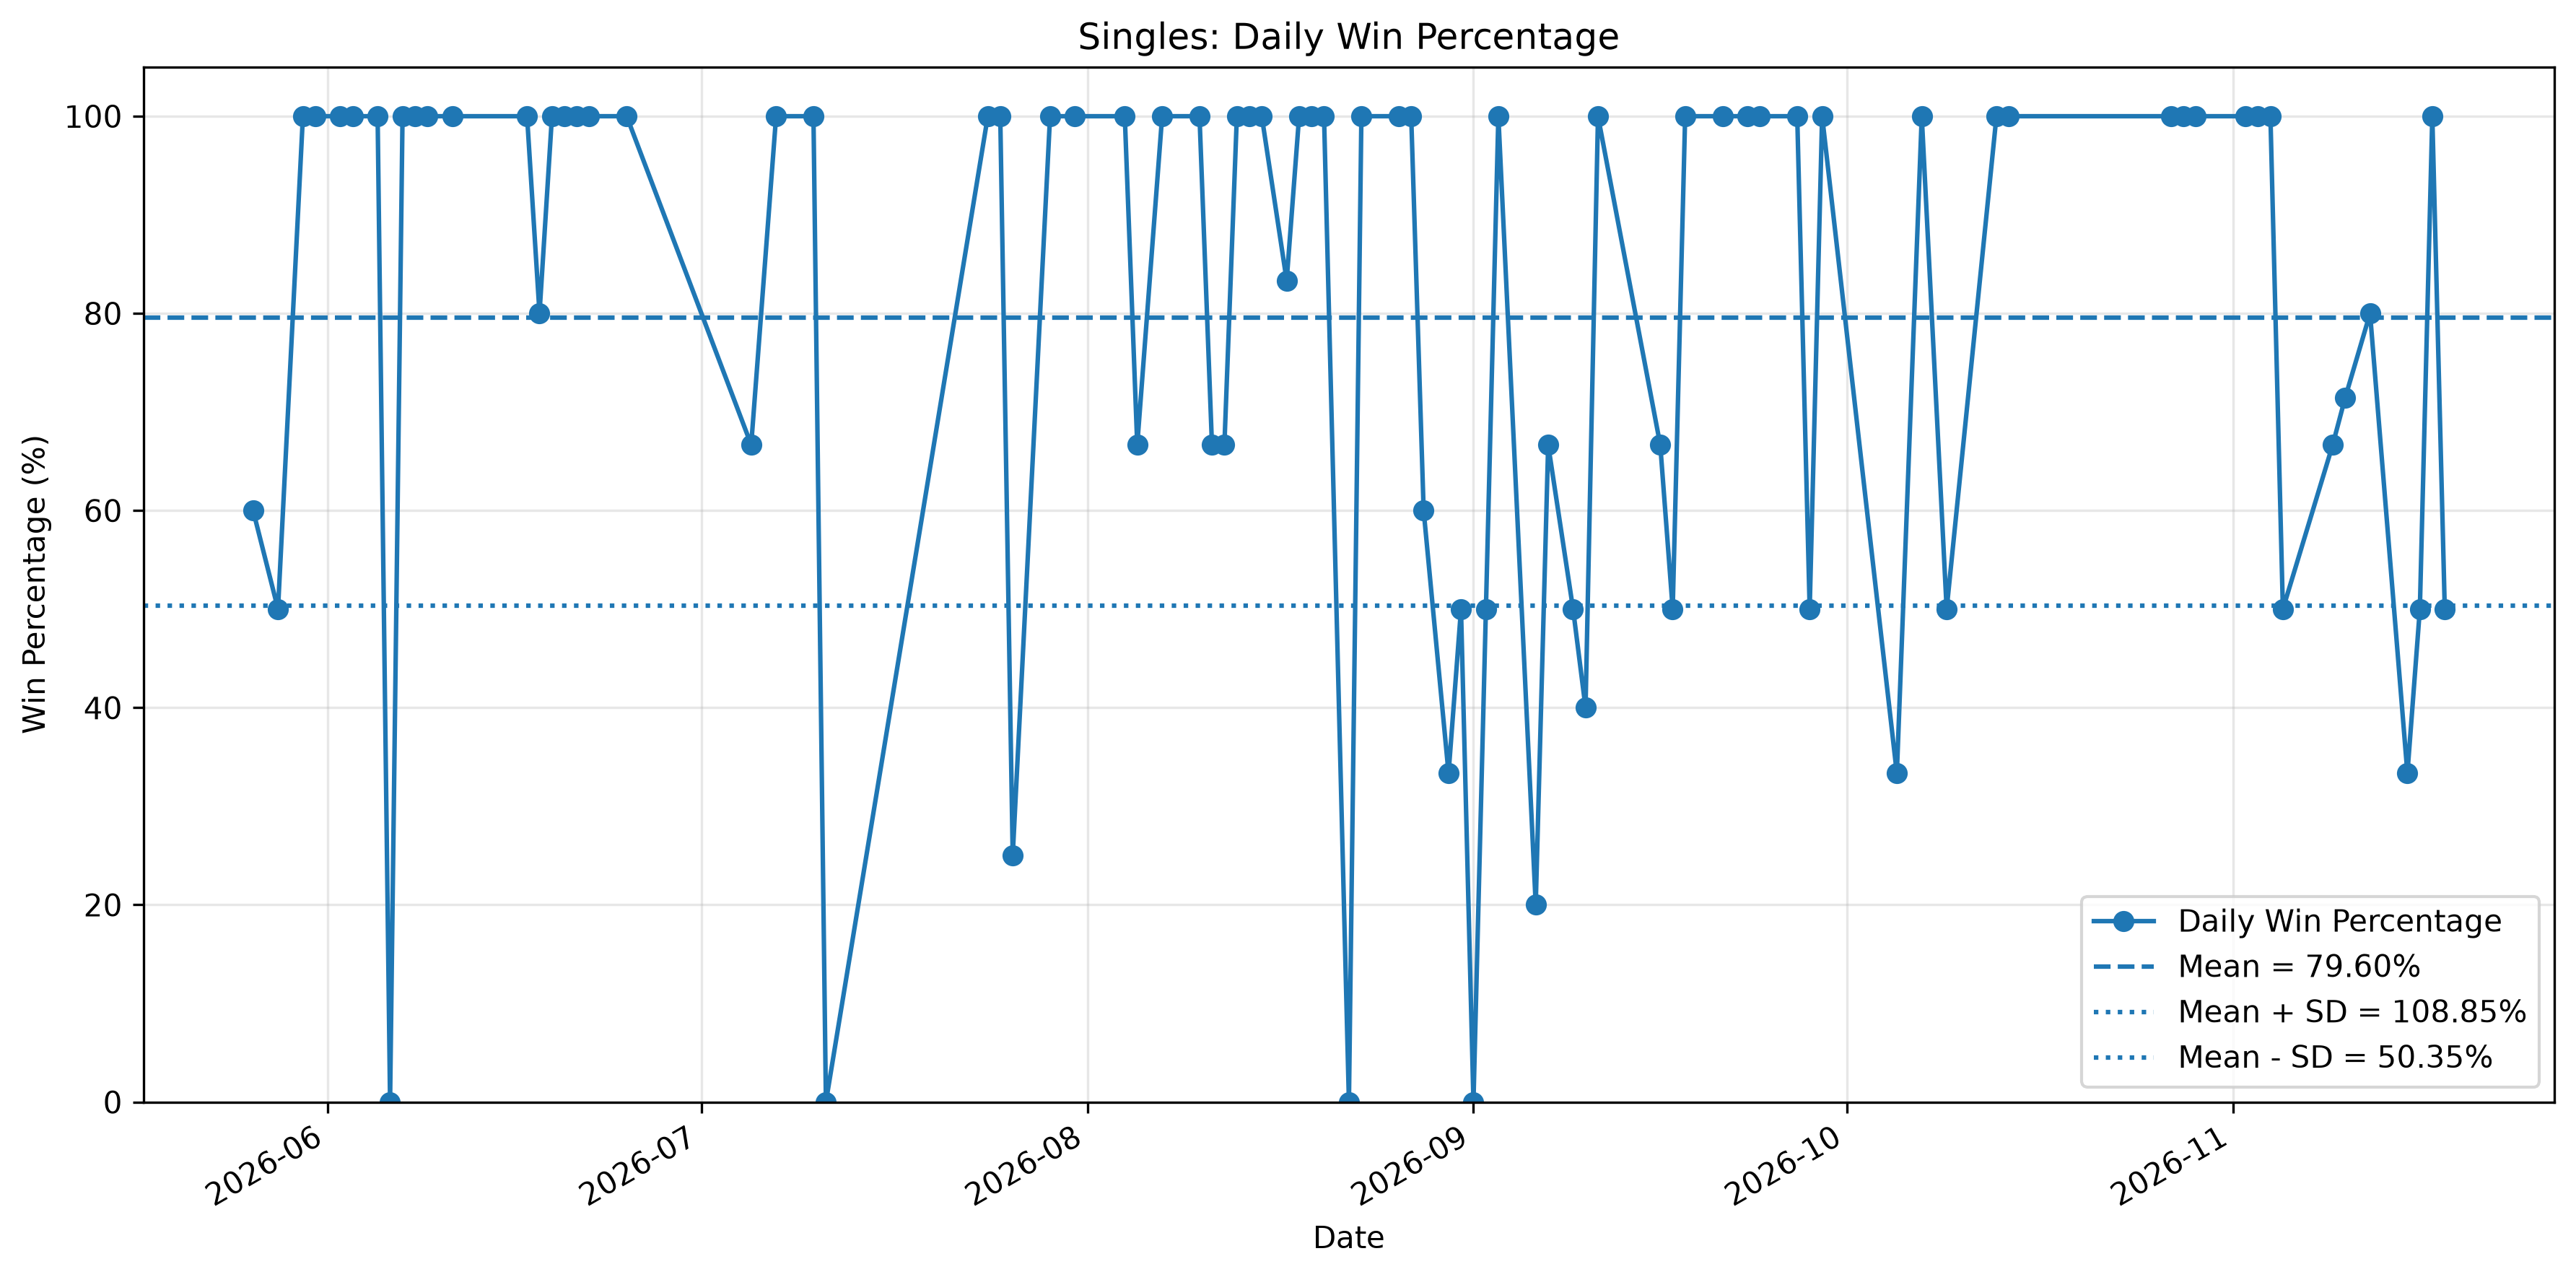
\includegraphics[width=0.96\textwidth]{figs/singles/daily_performance.png}
\caption{Daily performance for Singles.}
\label{fig:singles-daily_performance}
\end{figure}

\begin{figure}[H]
\centering
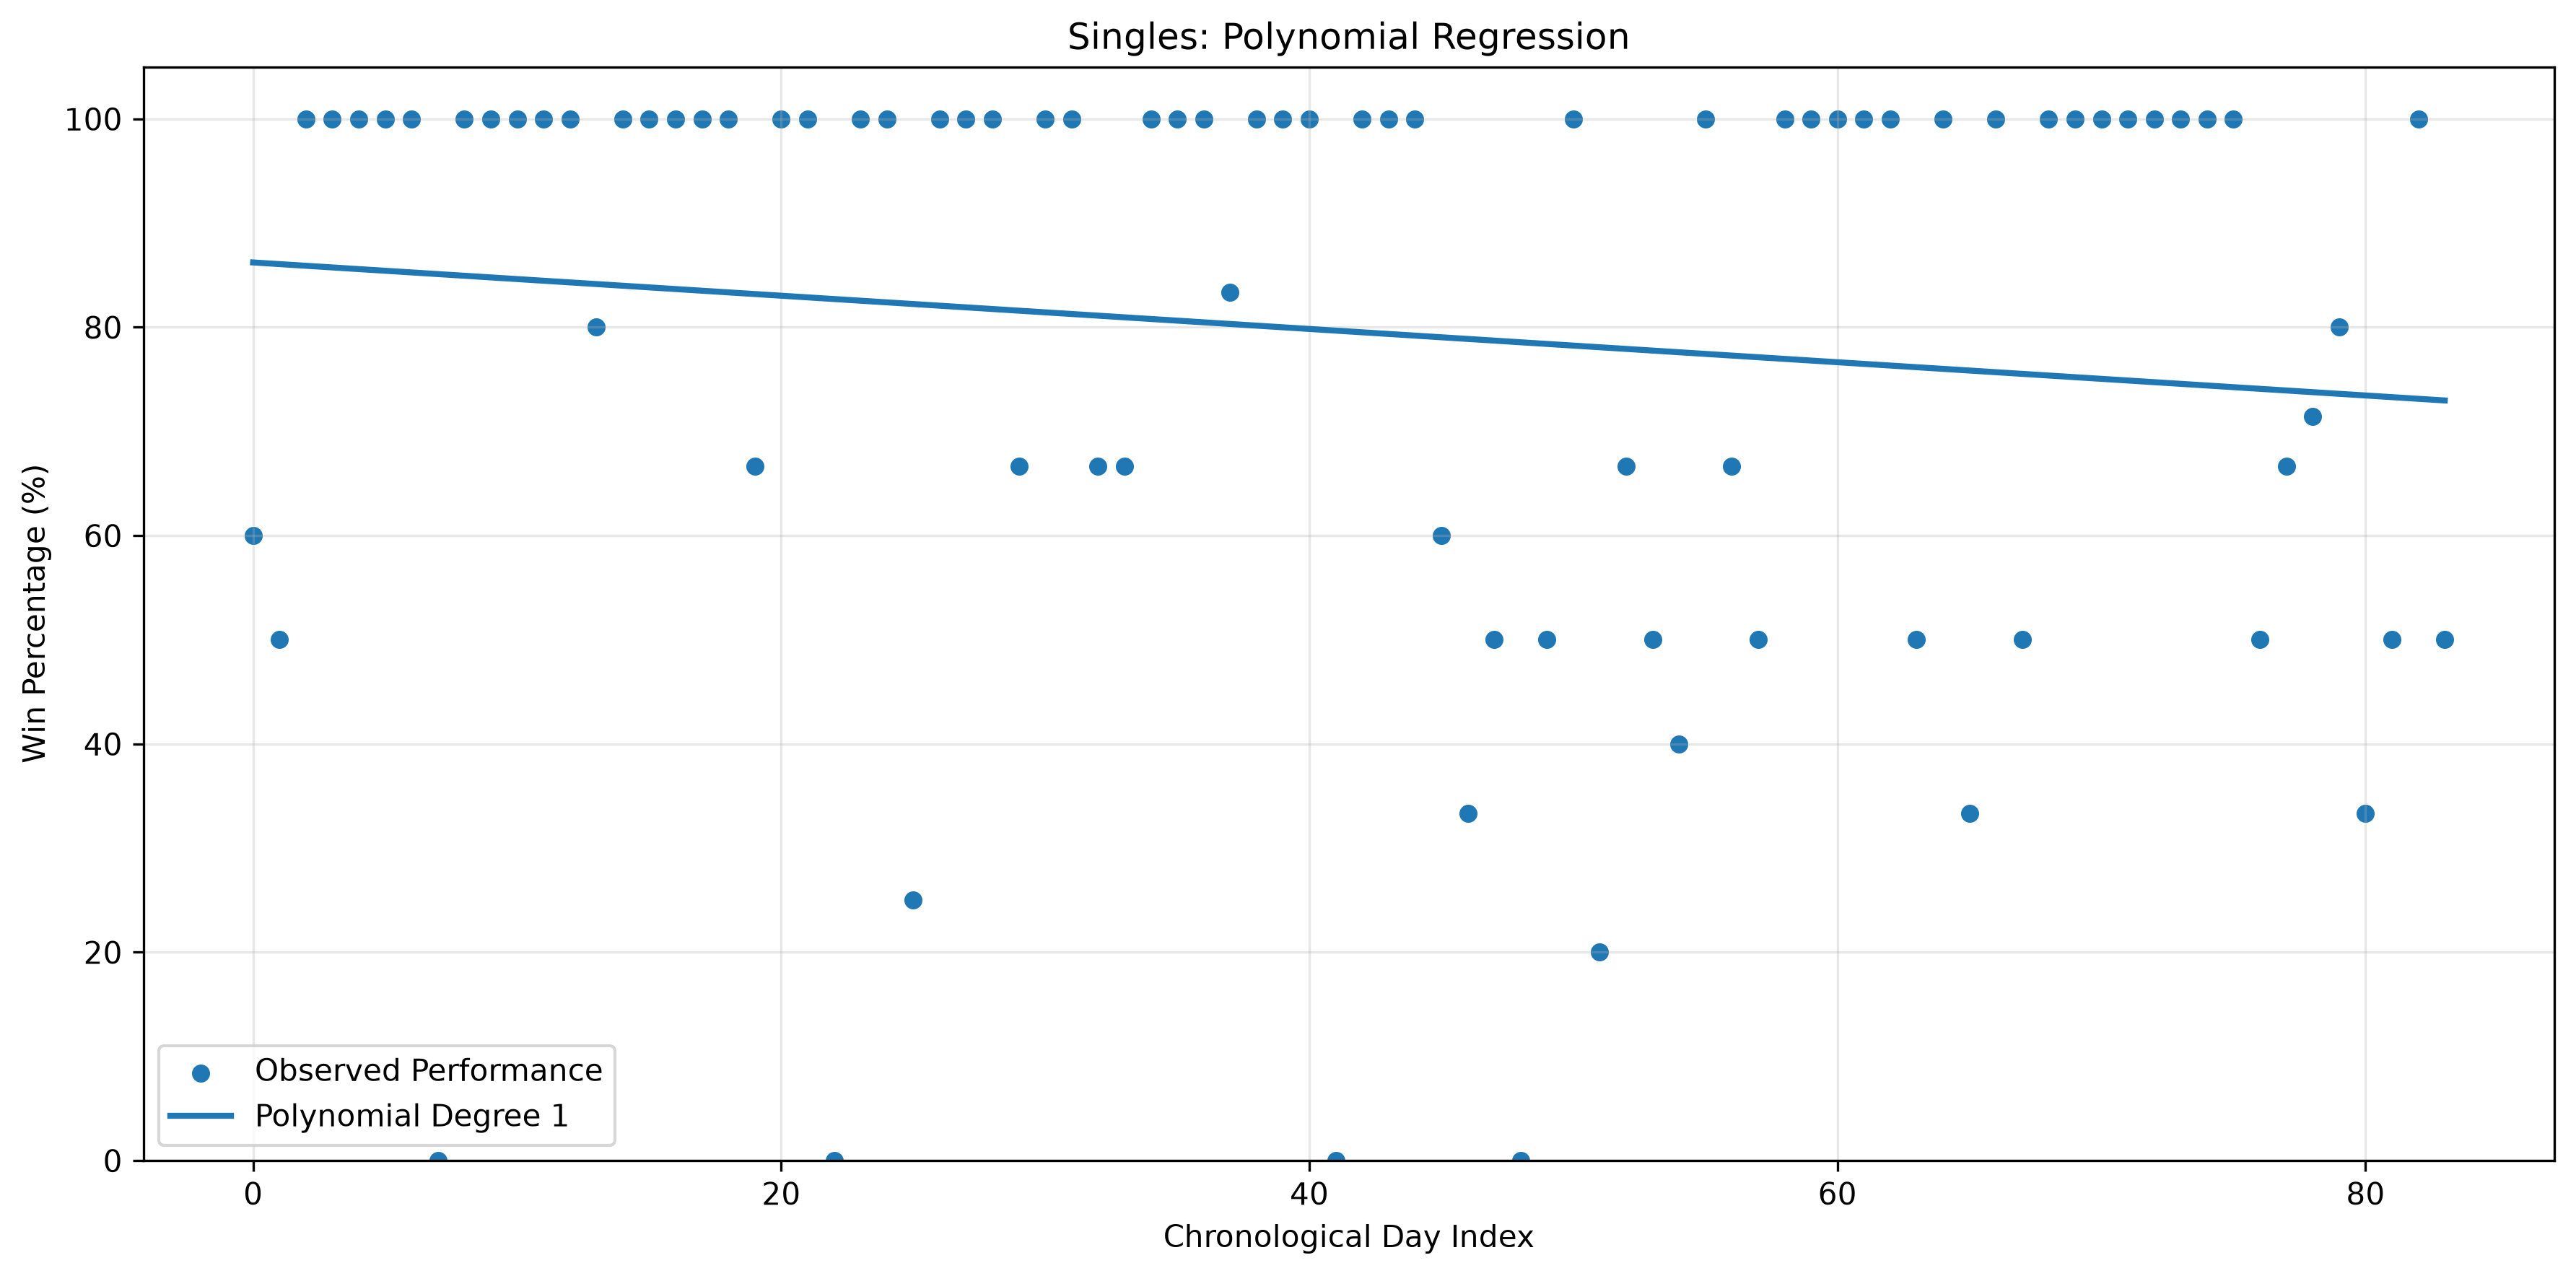
\includegraphics[width=0.96\textwidth]{figs/singles/polynomial_regression.png}
\caption{Regression fit for Singles.}
\label{fig:singles-polynomial_regression}
\end{figure}

\begin{figure}[H]
\centering
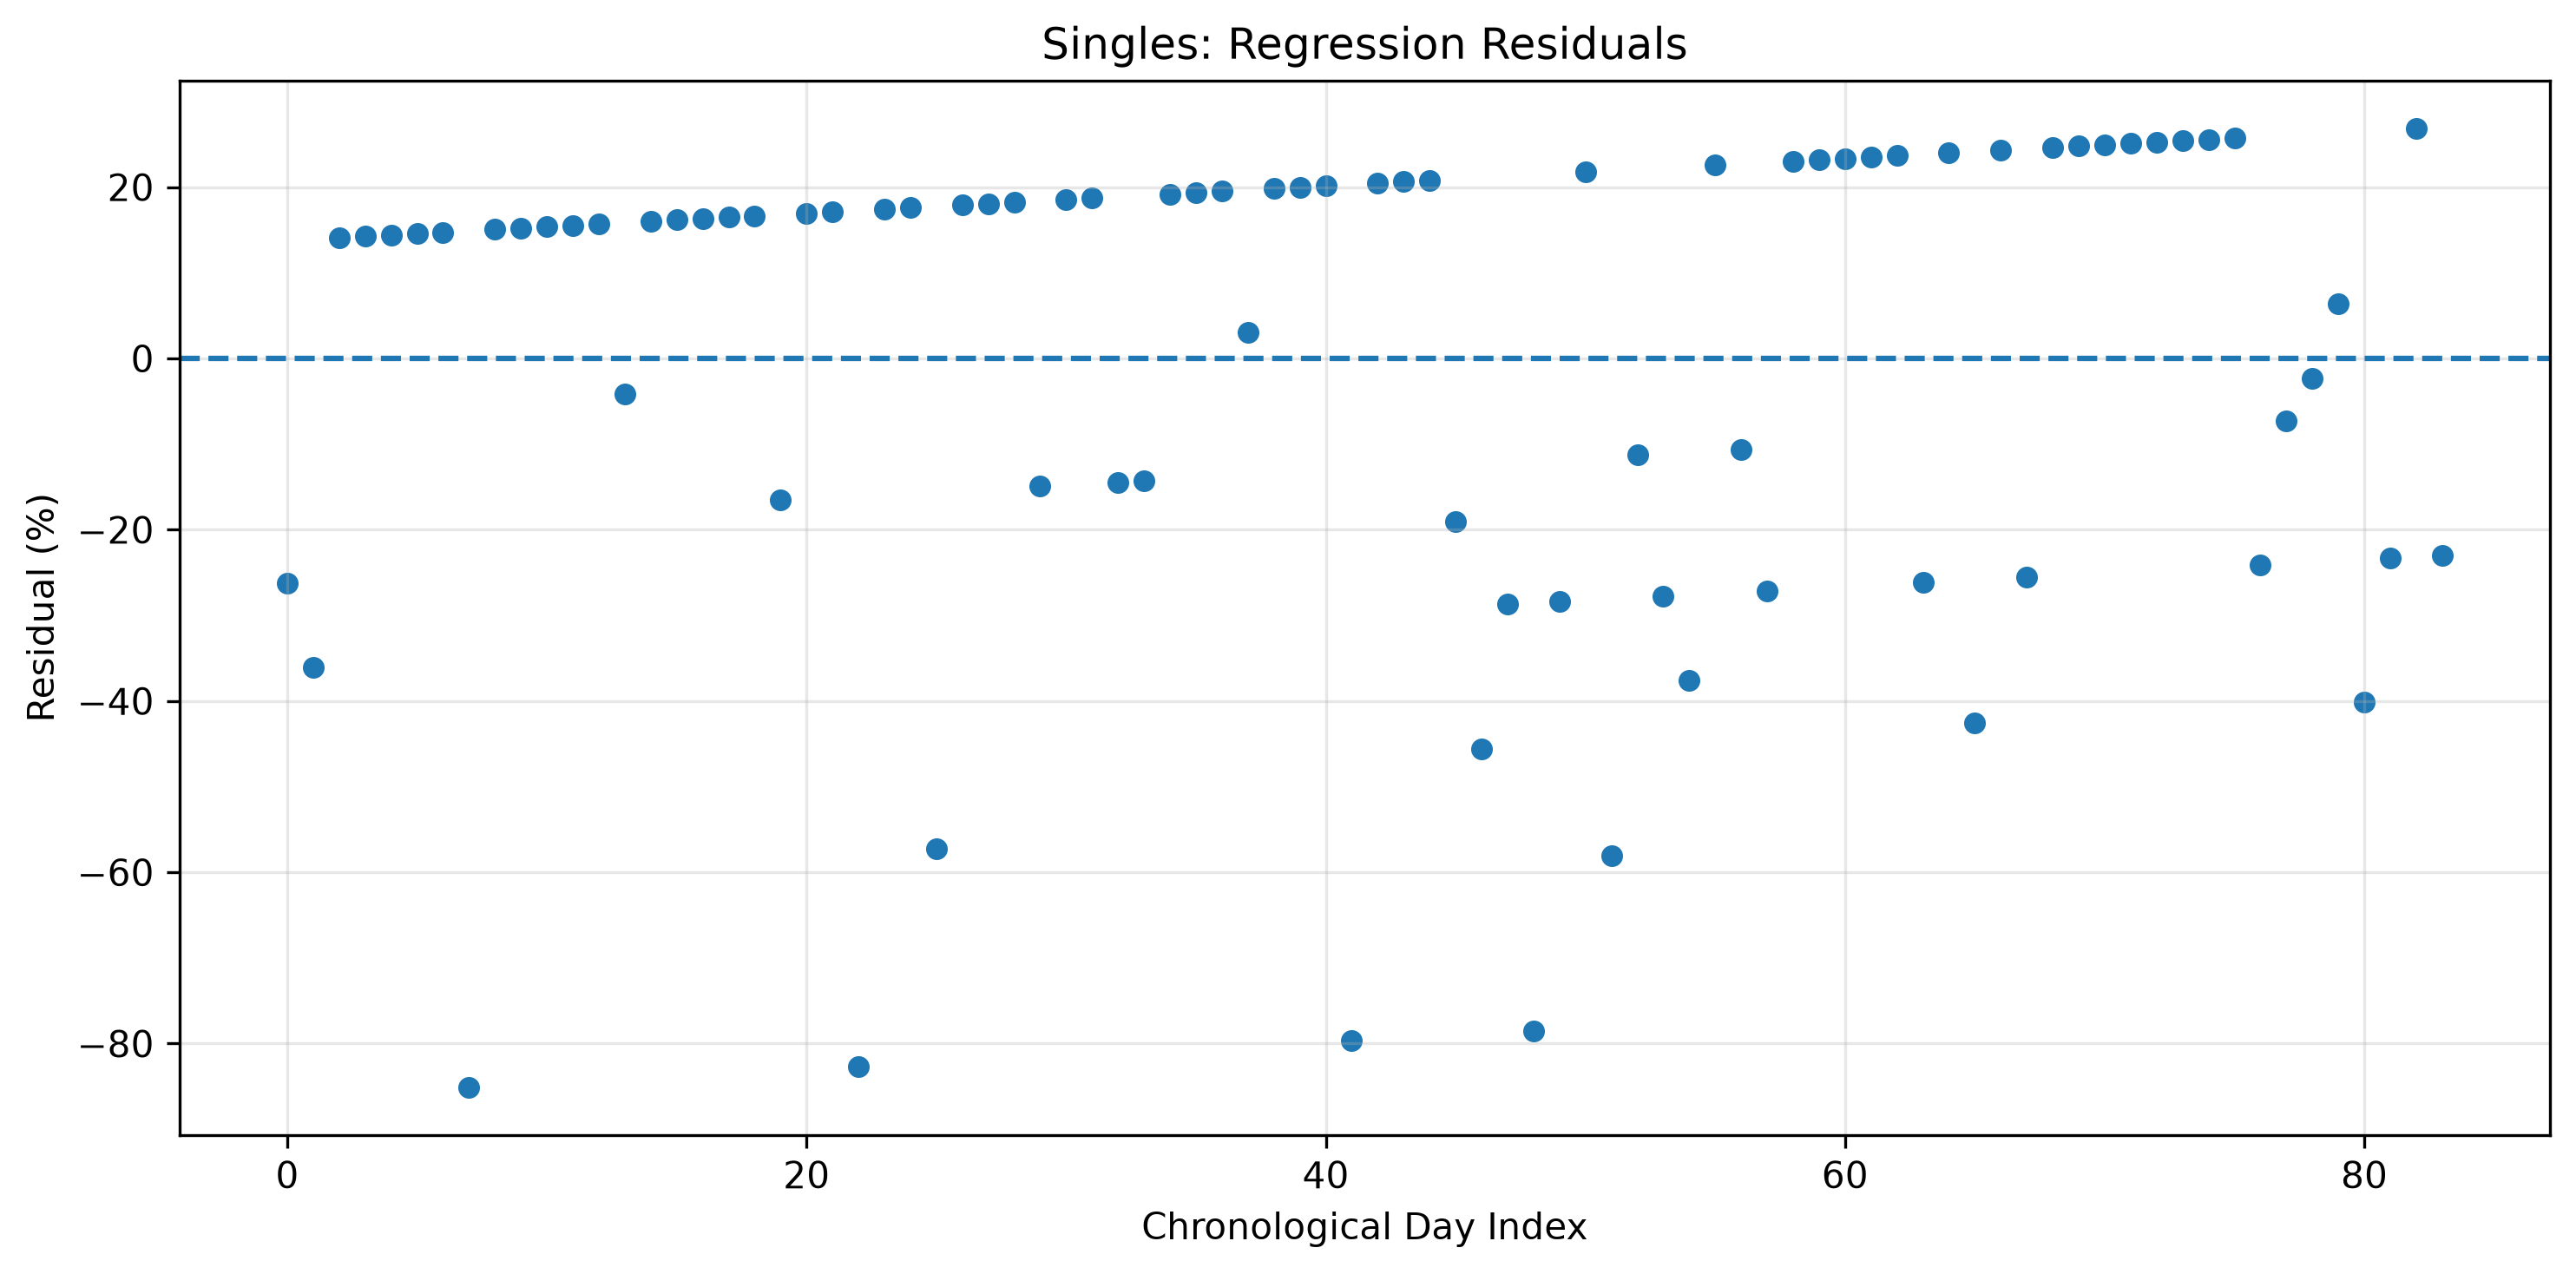
\includegraphics[width=0.96\textwidth]{figs/singles/regression_residuals.png}
\caption{Regression residuals for Singles.}
\label{fig:singles-regression_residuals}
\end{figure}

\subsection{Doubles}

\begin{figure}[H]
\centering
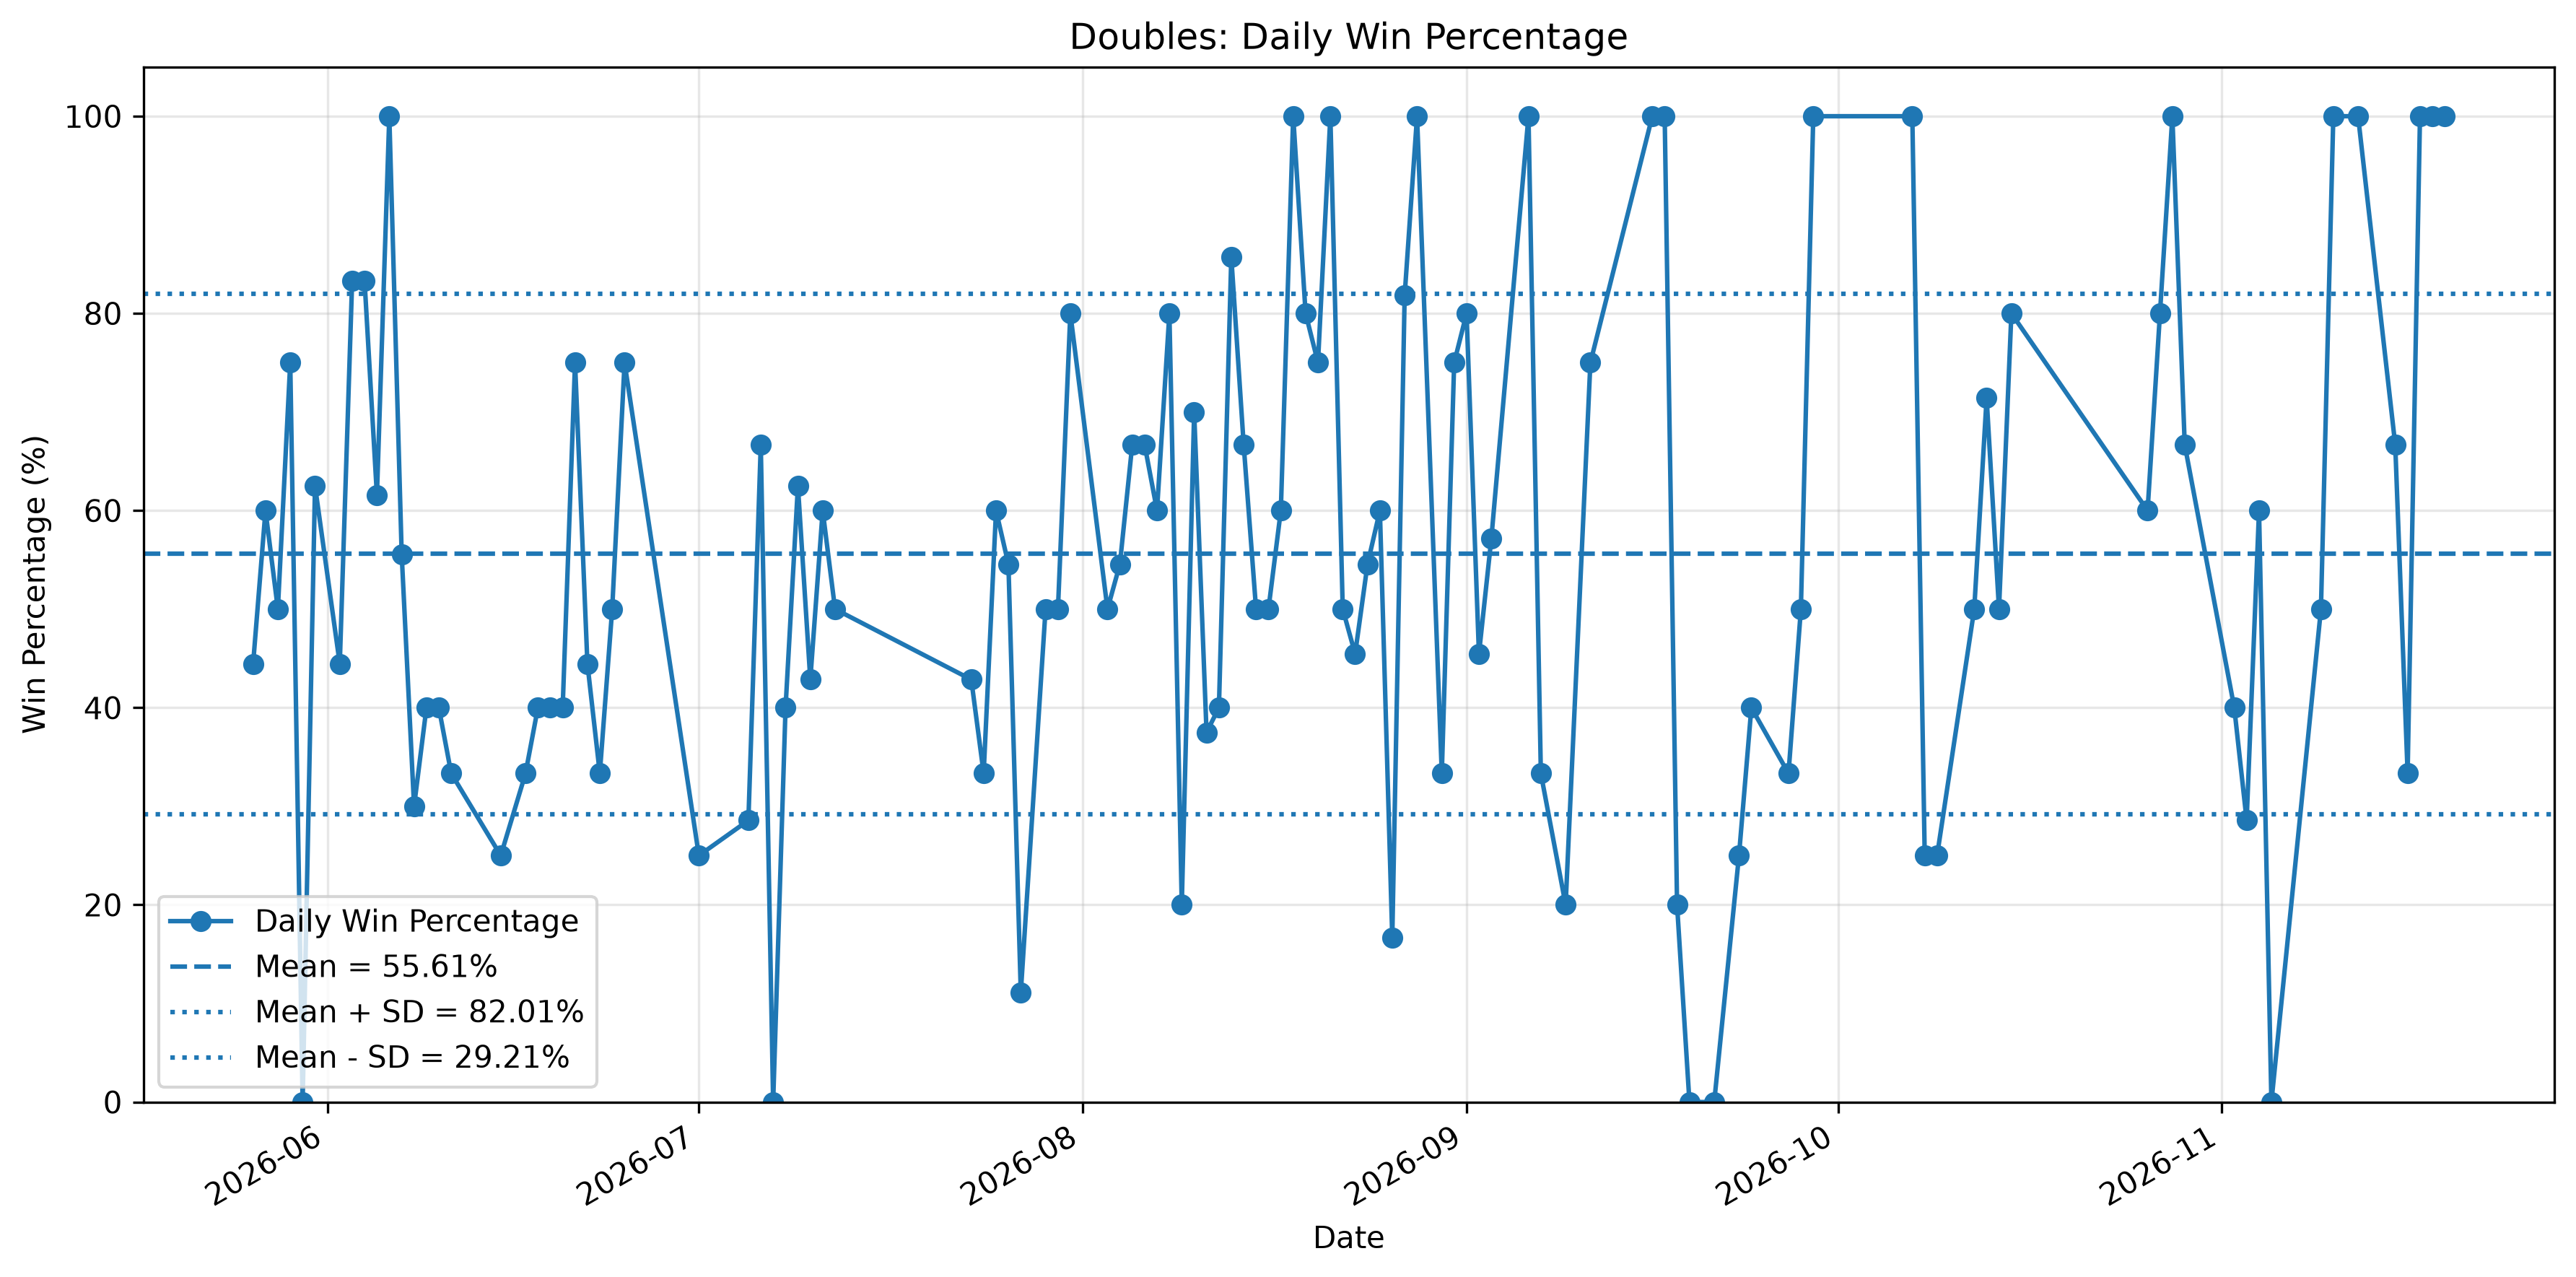
\includegraphics[width=0.96\textwidth]{figs/doubles/daily_performance.png}
\caption{Daily performance for Doubles.}
\label{fig:doubles-daily_performance}
\end{figure}

\begin{figure}[H]
\centering
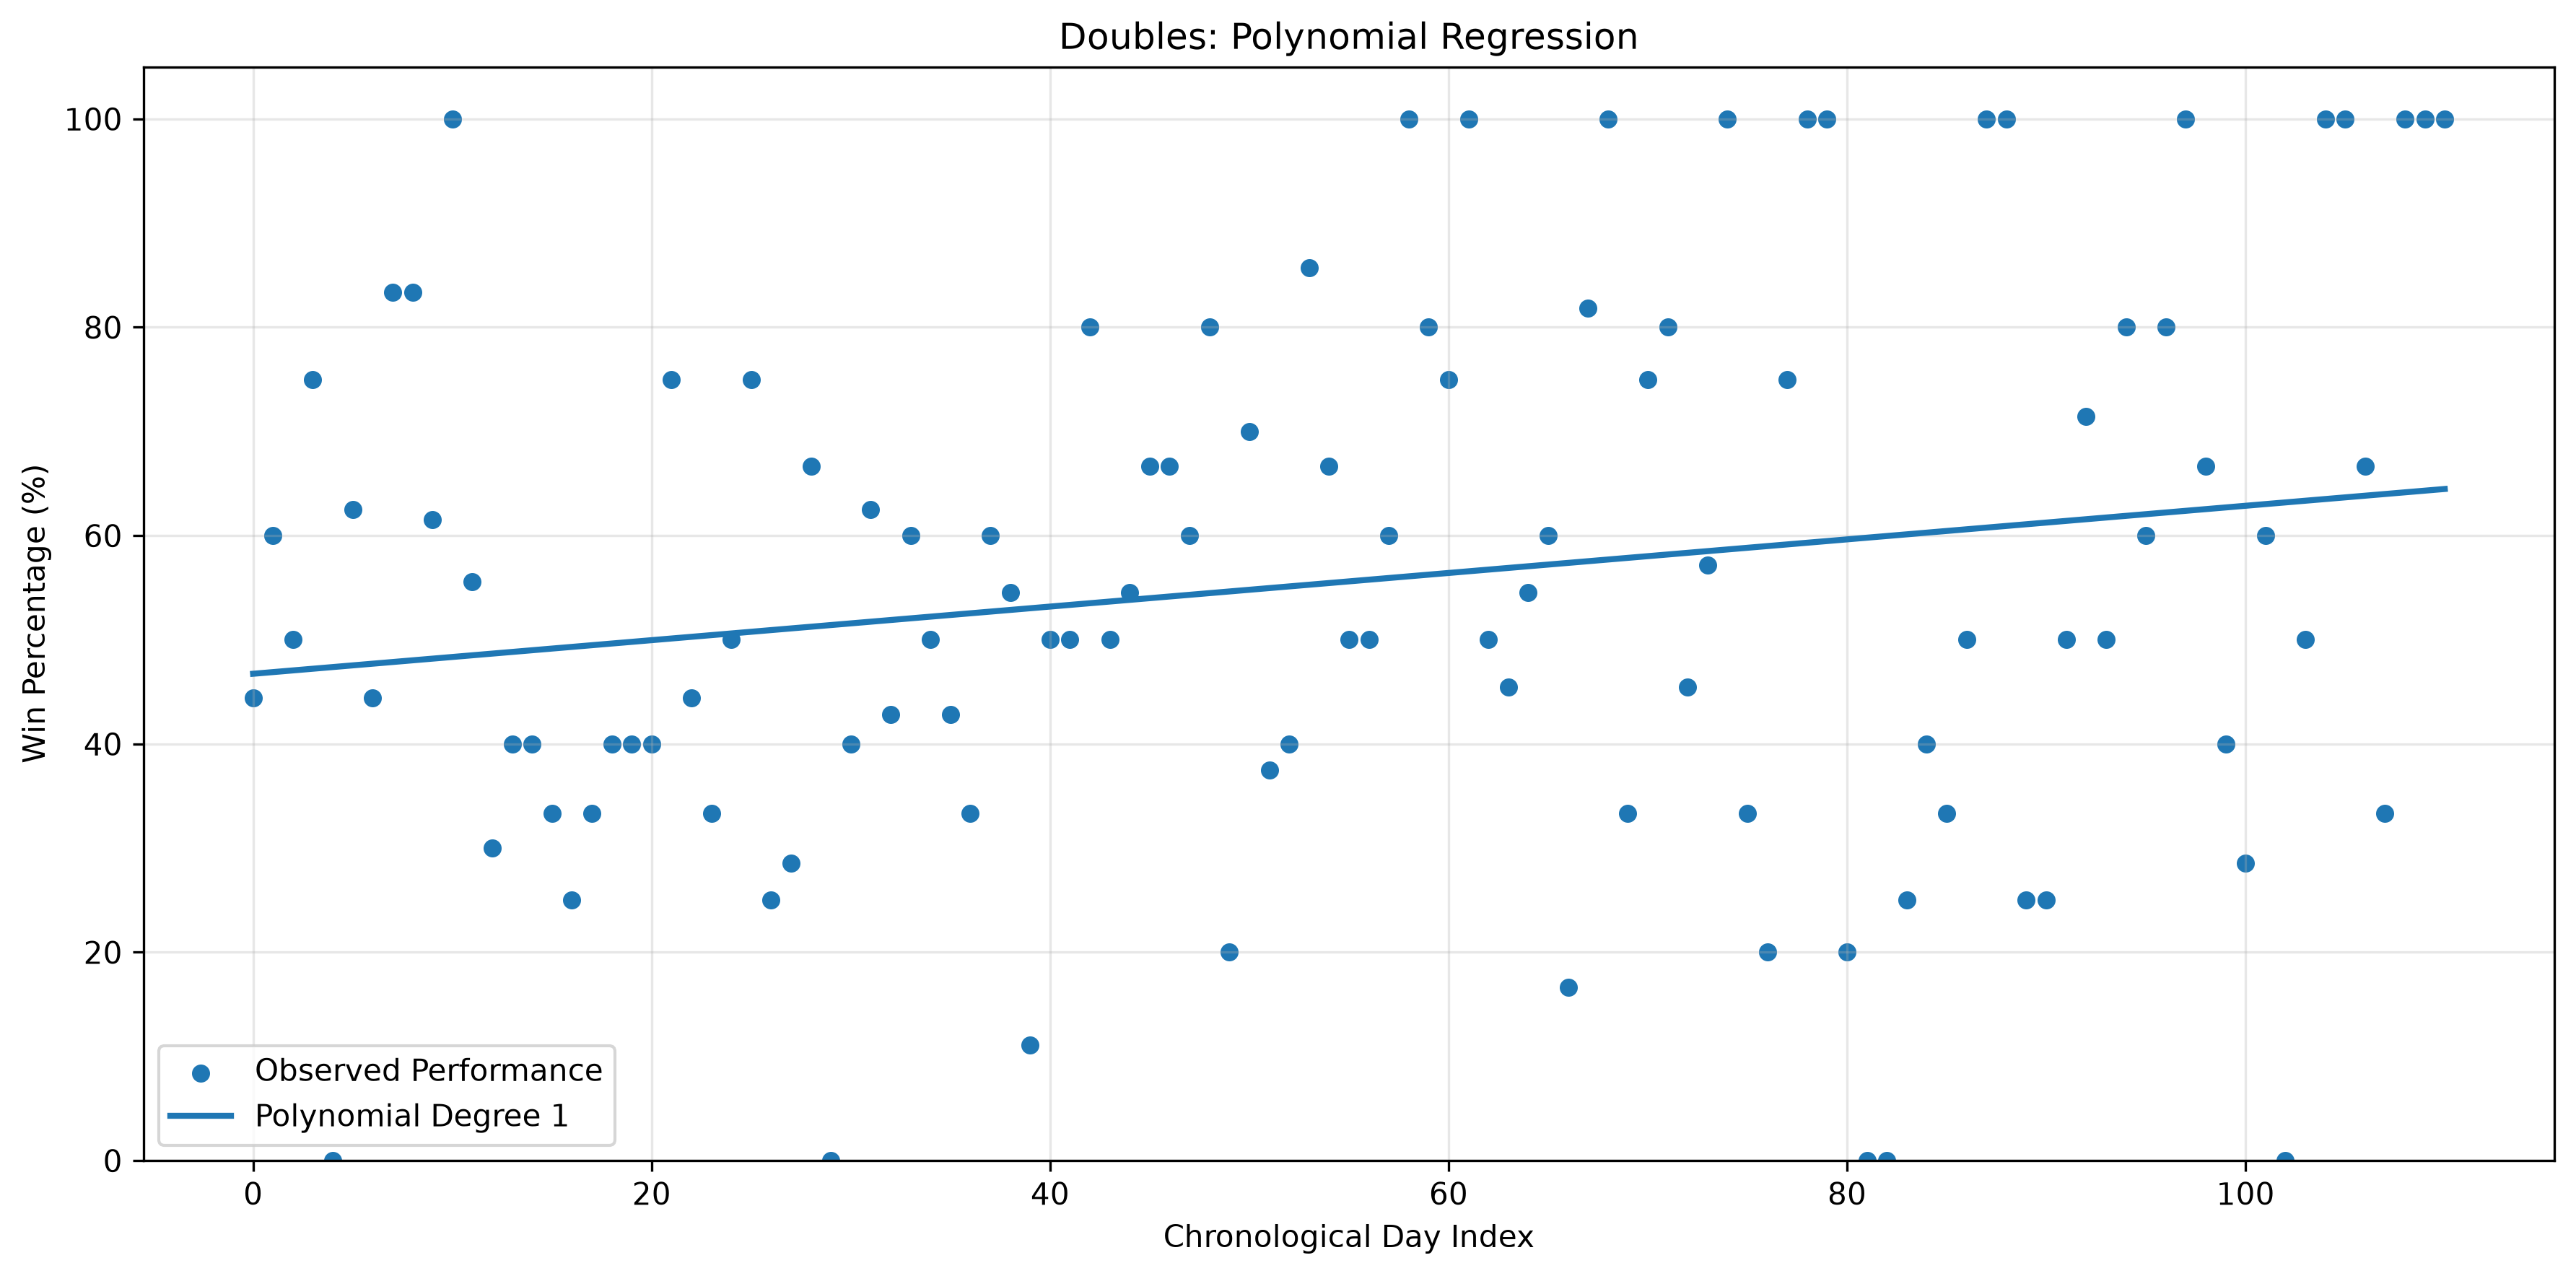
\includegraphics[width=0.96\textwidth]{figs/doubles/polynomial_regression.png}
\caption{Regression fit for Doubles.}
\label{fig:doubles-polynomial_regression}
\end{figure}

\begin{figure}[H]
\centering
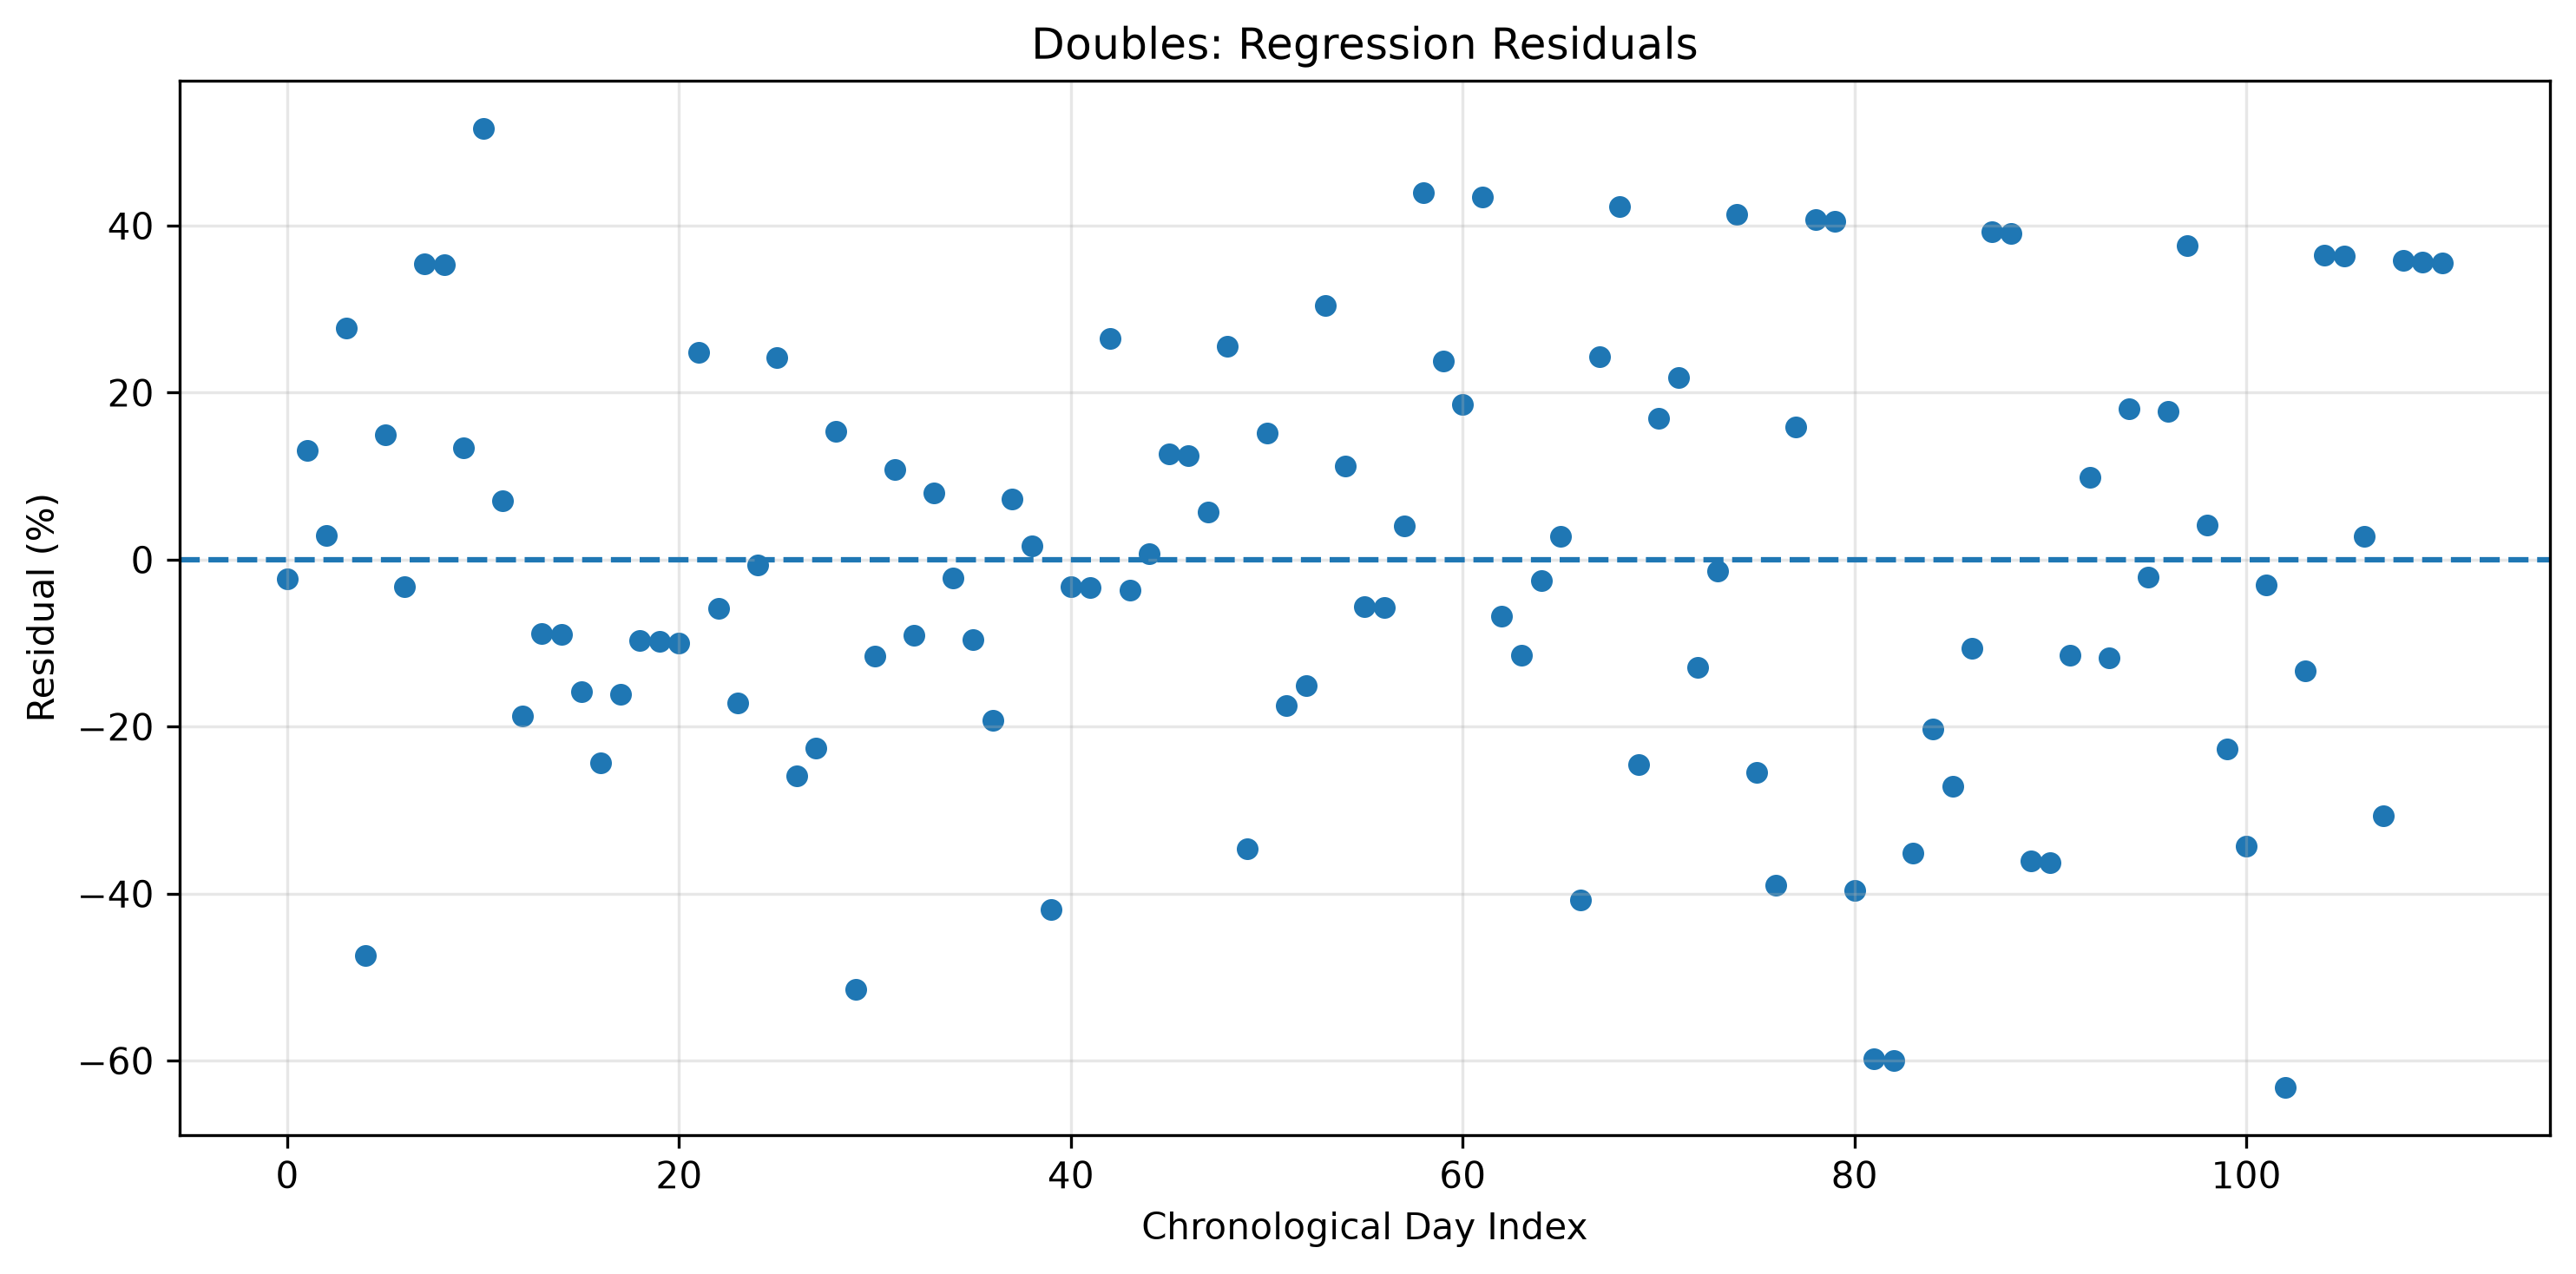
\includegraphics[width=0.96\textwidth]{figs/doubles/regression_residuals.png}
\caption{Regression residuals for Doubles.}
\label{fig:doubles-regression_residuals}
\end{figure}

\subsection{Mixed Doubles}

\begin{figure}[H]
\centering
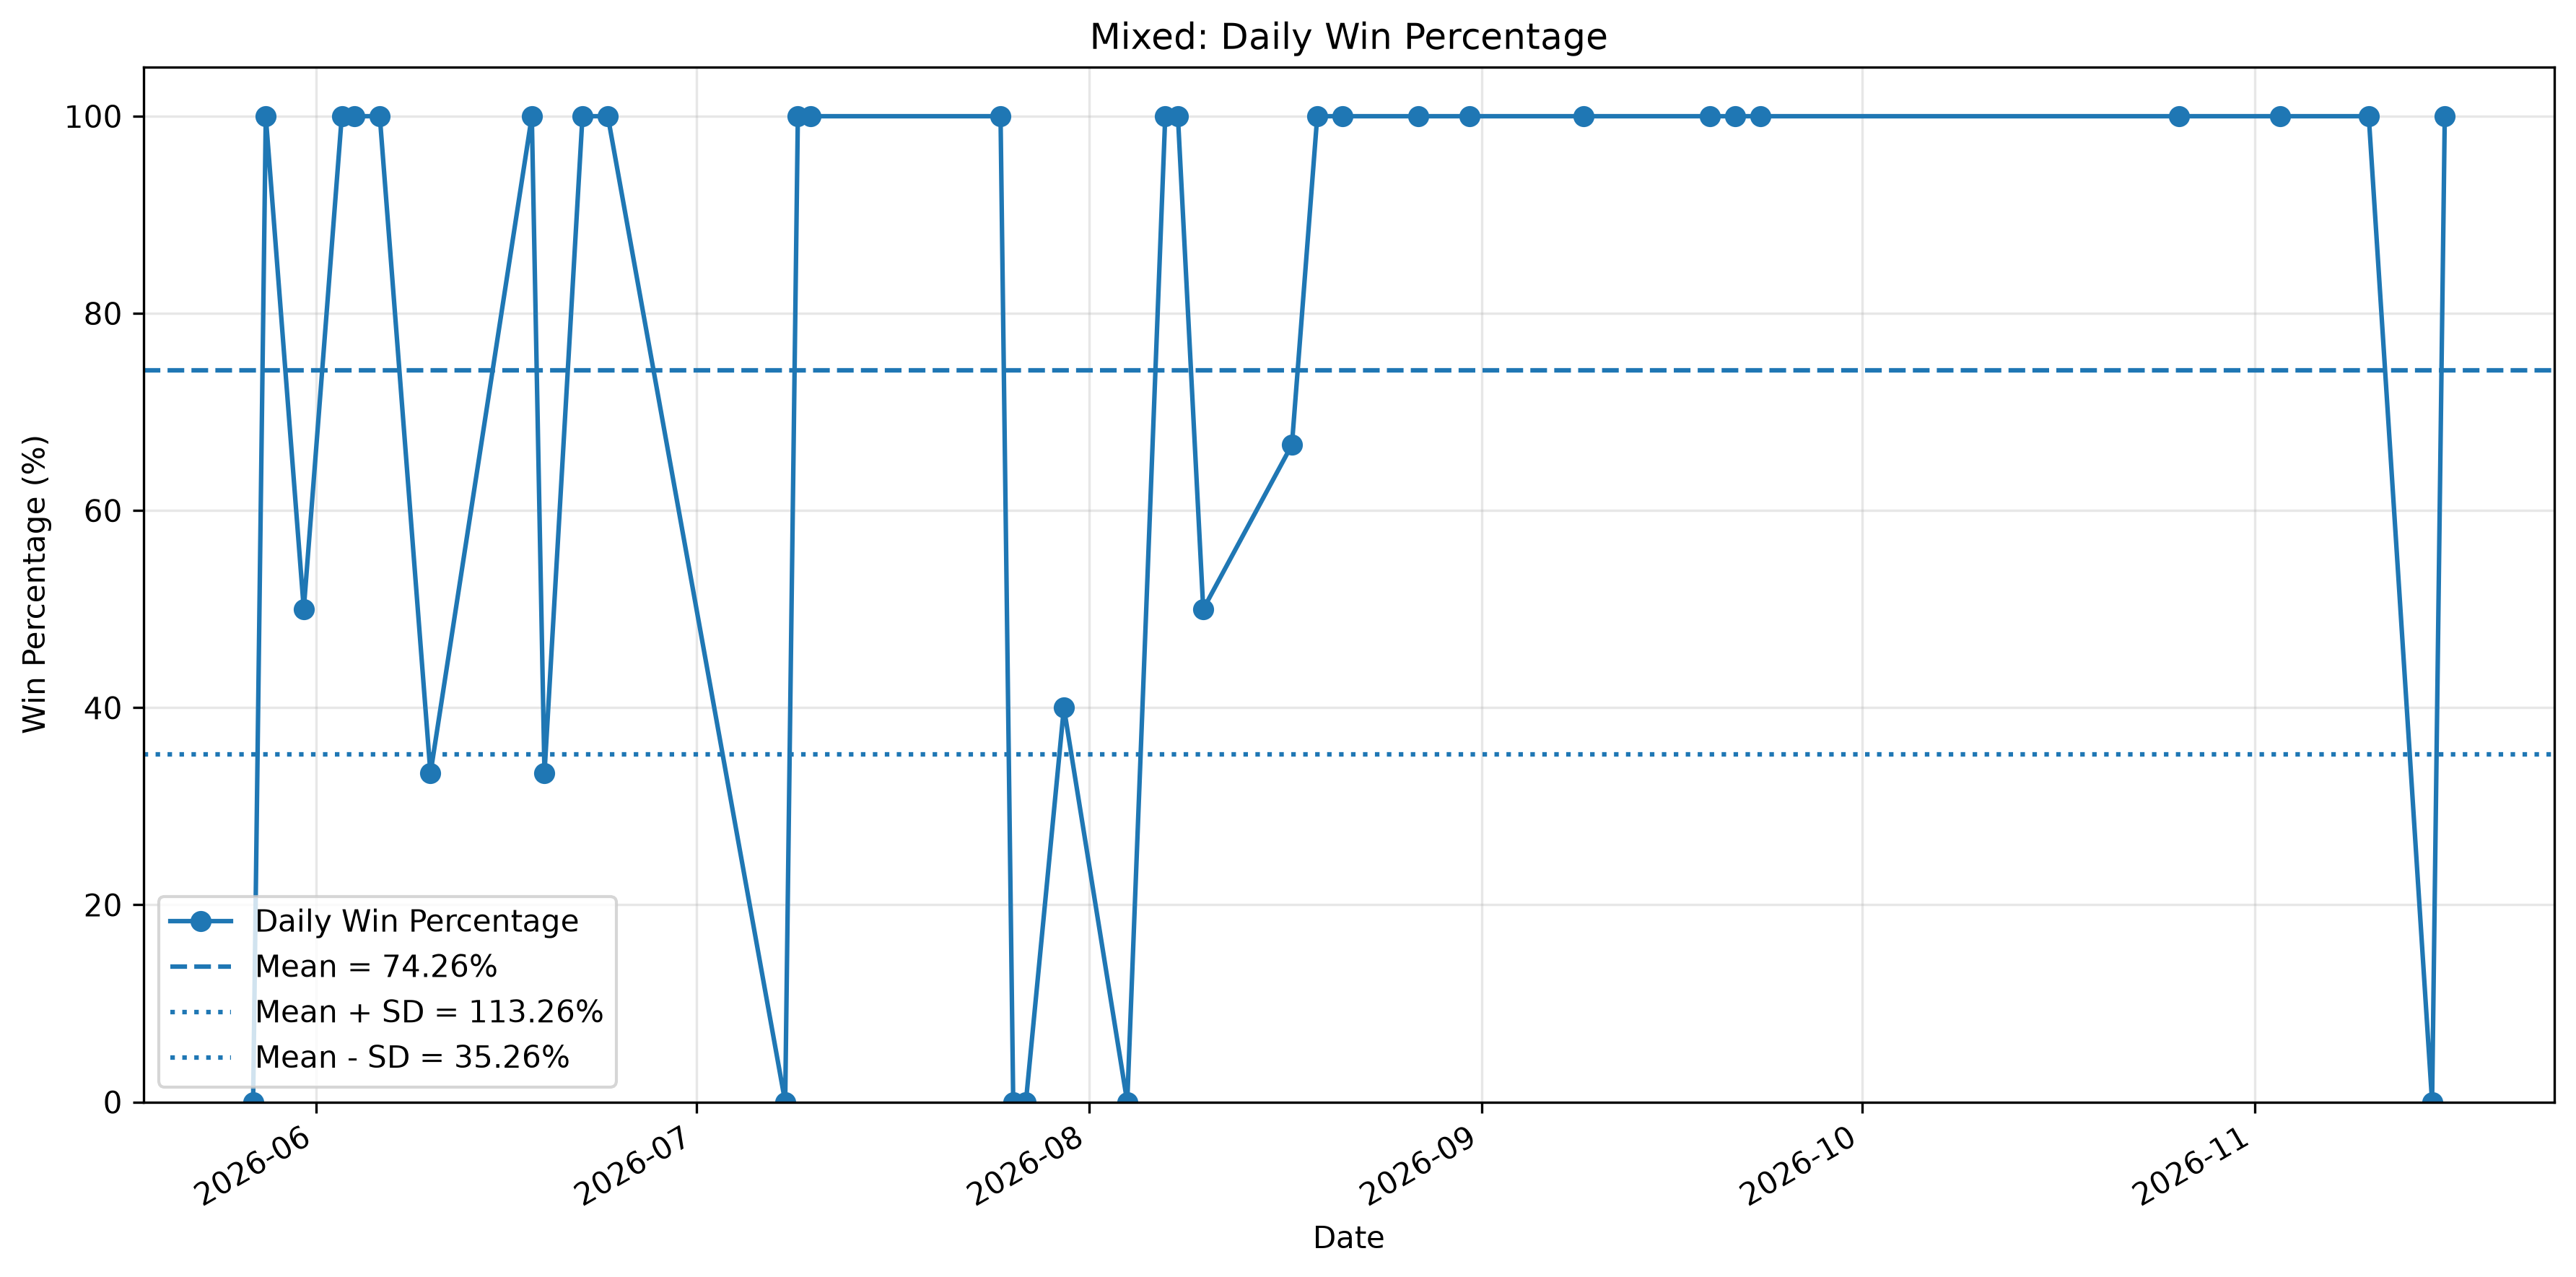
\includegraphics[width=0.96\textwidth]{figs/mixed/daily_performance.png}
\caption{Daily performance for Mixed.}
\label{fig:mixed-daily_performance}
\end{figure}

\begin{figure}[H]
\centering
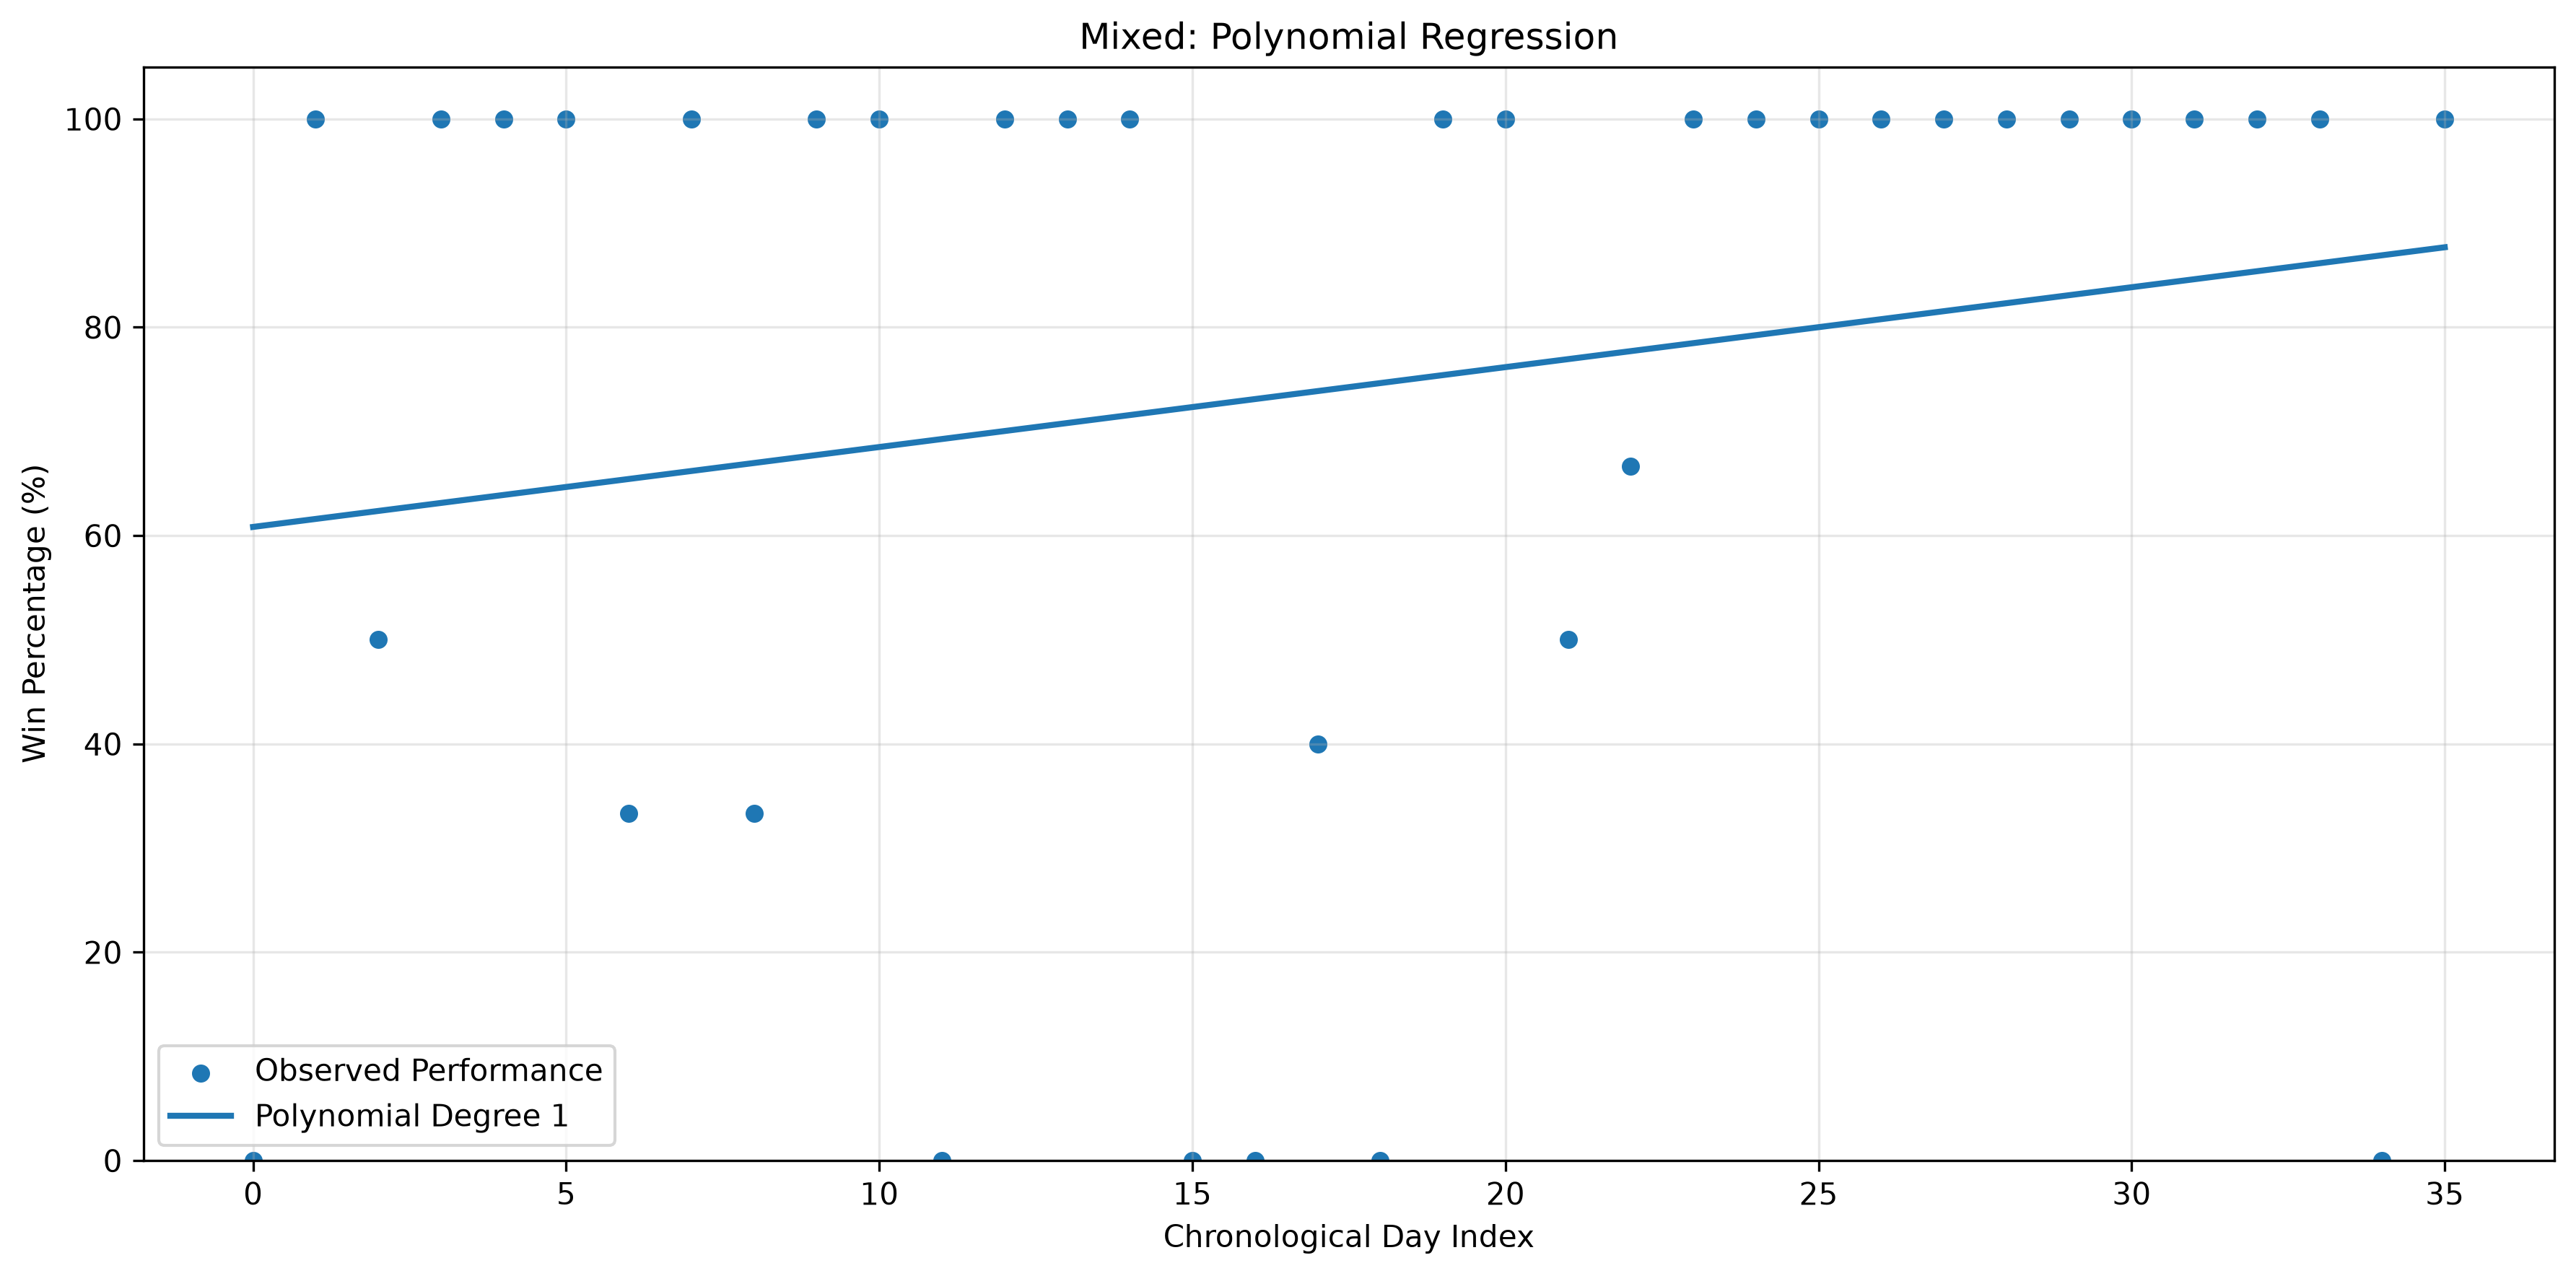
\includegraphics[width=0.96\textwidth]{figs/mixed/polynomial_regression.png}
\caption{Regression fit for Mixed.}
\label{fig:mixed-polynomial_regression}
\end{figure}

\begin{figure}[H]
\centering
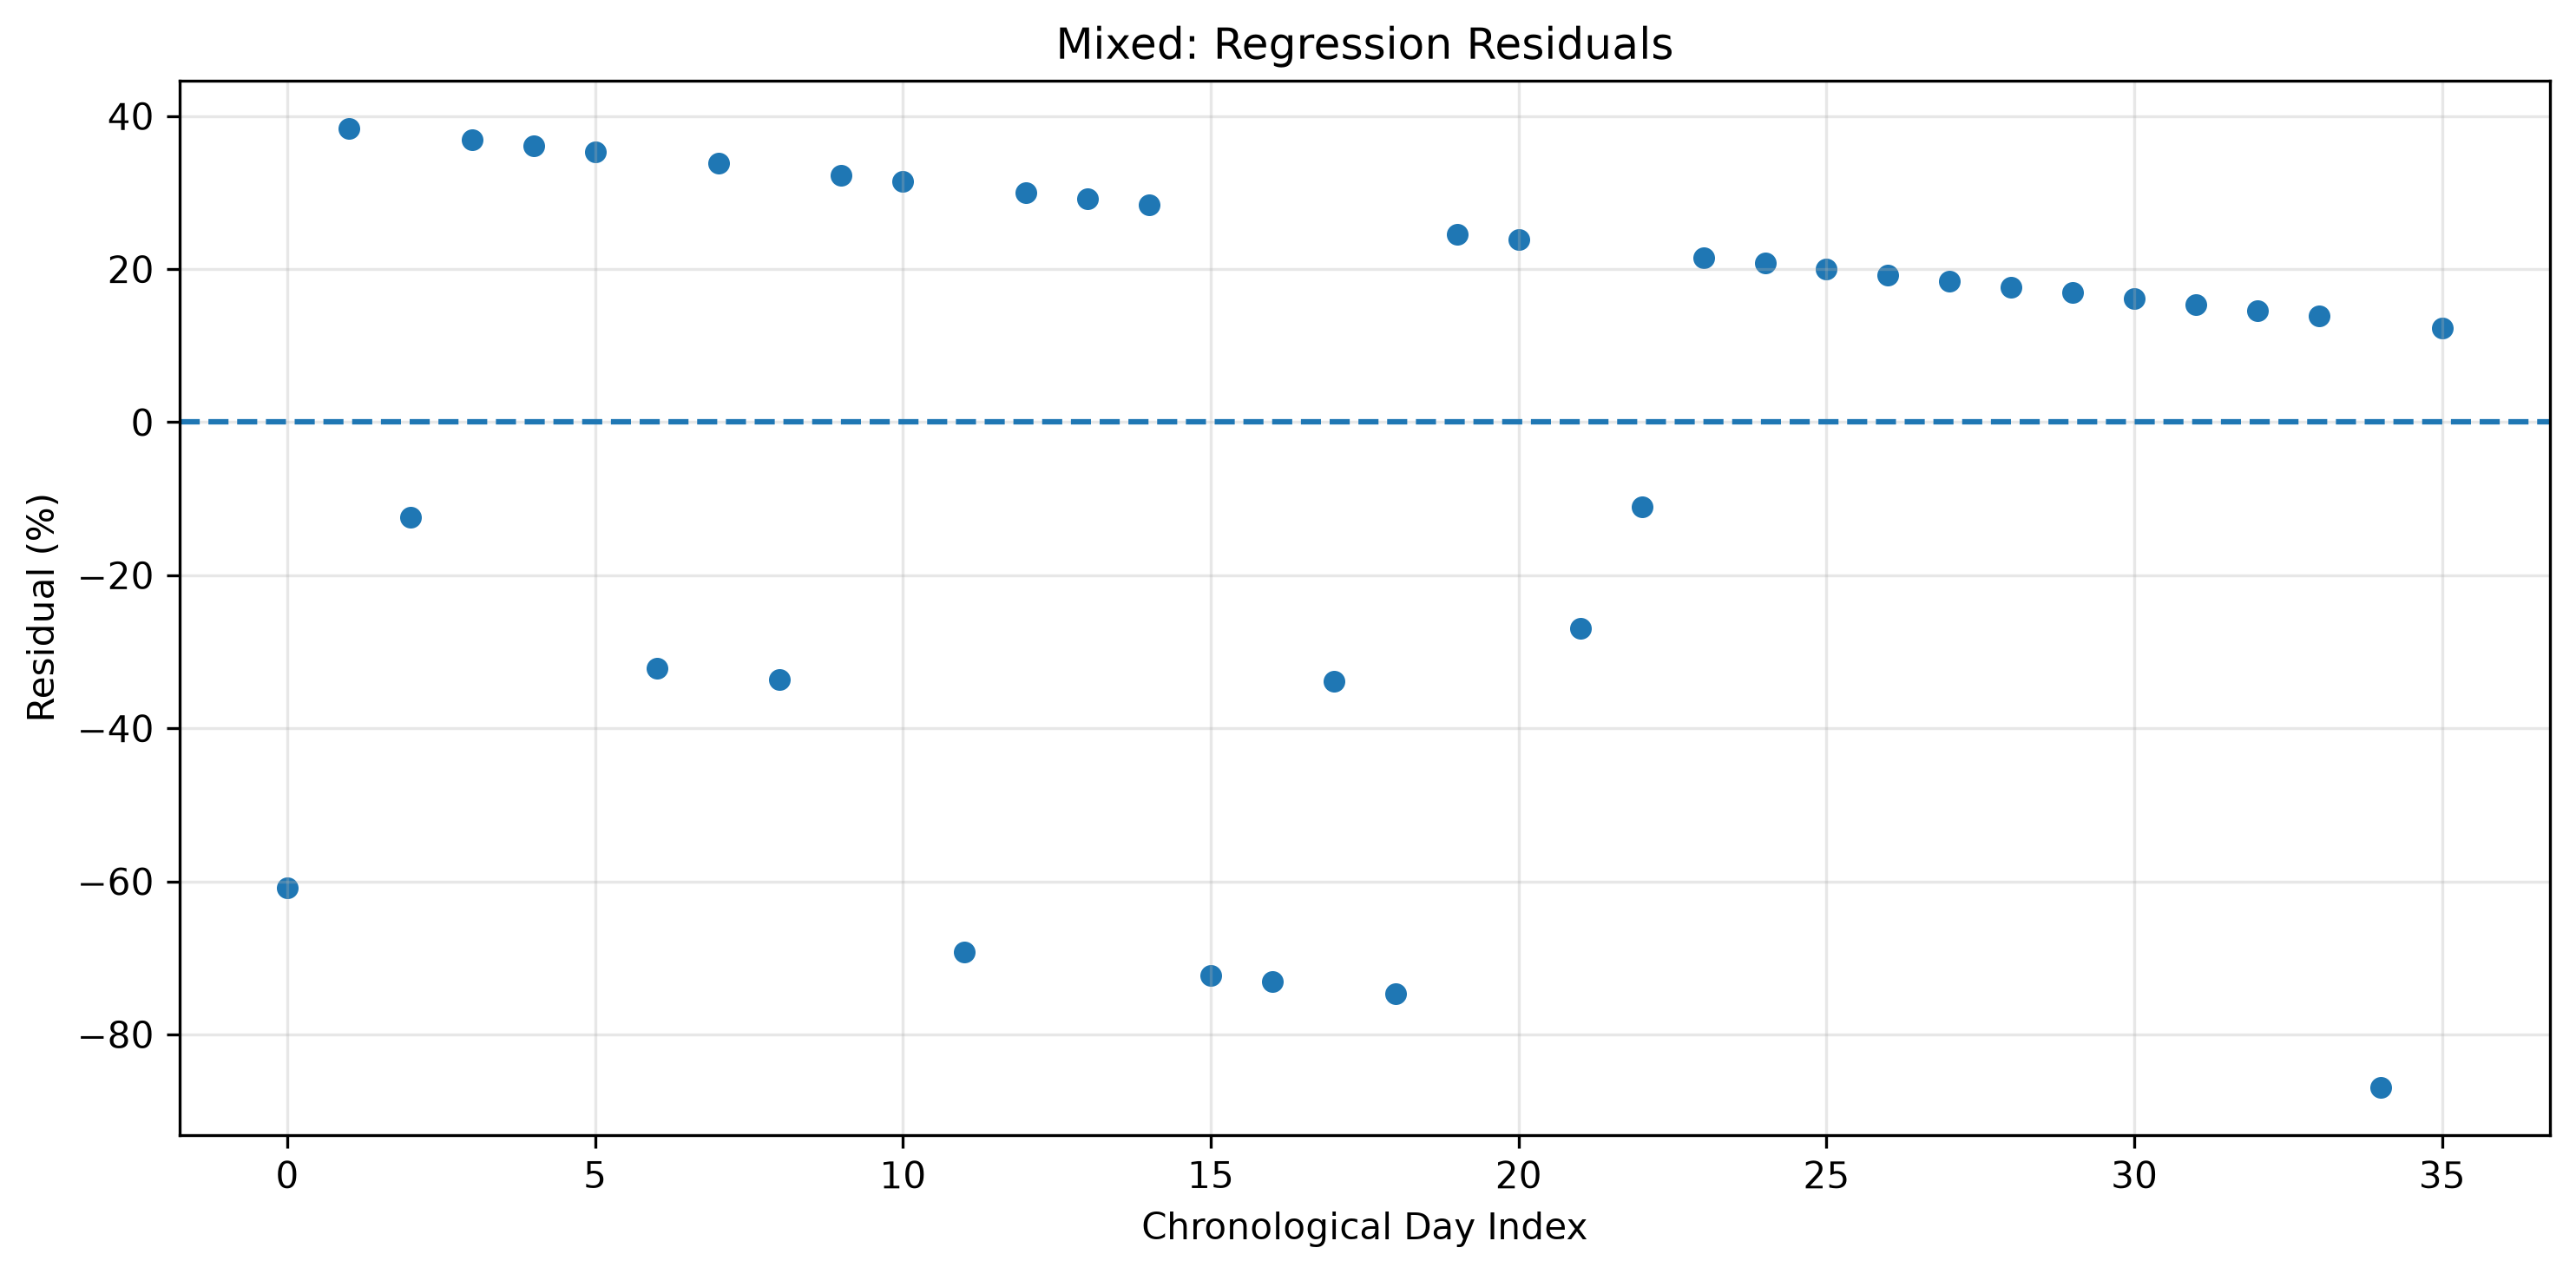
\includegraphics[width=0.96\textwidth]{figs/mixed/regression_residuals.png}
\caption{Regression residuals for Mixed.}
\label{fig:mixed-regression_residuals}
\end{figure}

% ============================================================
% 5. LEAST-SQUARES MODELLING
% ============================================================
\section{Least-Squares Modelling and Prediction}

\subsection{Why Linear Regression Was Selected}

The daily win percentages fluctuate considerably from one
playing day to another. The plotted observations do not show
a consistent repeating pattern or a clearly defined curved
relationship with time. Instead of forcing a complicated
curve through these fluctuations, a simple linear-regression
model is used as a first-order description of the overall
historical direction.

Linear regression was selected for three practical reasons.
First, its equation and coefficients are straightforward to
interpret. Second, it provides a transparent baseline against
which the observed percentages can be compared. Third, higher-
order polynomial and more advanced time-series methods are
outside the scope of this assignment. Such methods would add
complexity and, with a noisy record, could fit random
fluctuations rather than a stable underlying pattern.

The line is therefore not claimed to capture every rise and
fall. It summarizes the broad direction, if one exists, across
the recorded playing days.

\subsection{Linear Model and Least-Squares Derivation}

Let \(x_i\) be the chronological index of the \(i\)-th
recorded playing day and let \(P_i\) be its daily win
percentage. The linear model is

\begin{equation}
\widehat{P}(x)=a+bx,
\label{eq:linear-model}
\end{equation}

where \(a\) is the intercept and \(b\) is the slope. The
slope represents the estimated change in win percentage, in
percentage points, for one additional recorded playing day.

The coefficients are chosen to minimize the sum of squared
residuals:

\begin{equation}
S(a,b)=\sum_{i=1}^{n}\left[P_i-(a+bx_i)\right]^2.
\label{eq:least-squares-objective}
\end{equation}

For the matrix representation, define

\[
\mathbf{X}=\begin{bmatrix}
1 & x_1\\
1 & x_2\\
\vdots & \vdots\\
1 & x_n
\end{bmatrix},\qquad
\mathbf{a}=\begin{bmatrix}a\\b\end{bmatrix},\qquad
\mathbf{P}=\begin{bmatrix}P_1\\P_2\\\vdots\\P_n\end{bmatrix}.
\]

The fitted values are \(\widehat{\mathbf{P}}=\mathbf{X}\mathbf{a}\),
and the least-squares problem becomes

\begin{equation}
\min_{\mathbf{a}}\left\|\mathbf{P}-\mathbf{X}\mathbf{a}\right\|_2^2.
\label{eq:matrix-least-squares}
\end{equation}

The normal equations are

\begin{equation}
\mathbf{X}^{T}\mathbf{X}\mathbf{a}=\mathbf{X}^{T}\mathbf{P}.
\label{eq:normal-equations}
\end{equation}

When the columns of \(\mathbf{X}\) are linearly independent,
the coefficient estimate can be written as

\begin{equation}
\mathbf{a}=(\mathbf{X}^{T}\mathbf{X})^{-1}
\mathbf{X}^{T}\mathbf{P}.
\label{eq:coefficient-solution}
\end{equation}

In numerical computation, a least-squares routine is
preferable to explicitly calculating the matrix inverse.

\subsection{Implementation}

The Python implementation fits a straight line separately
for Singles, Doubles and Mixed Doubles using the chronological
playing-day index as the independent variable and daily win
percentage as the dependent variable. The three formats are
fitted independently because their sample sizes and match
patterns differ.

The fitted line is plotted with the observed percentages.
A corresponding residual plot is also generated for each
format. The implementation and figure generation code path is
listed in Appendix~\ref{app:python-implementation}.

\subsection{Residuals and Model Evaluation}

The residual at observation \(i\) is the difference between
the actual daily percentage and the value predicted by the
fitted line:

\begin{equation}
e_i=P_i-\widehat{P}(x_i).
\label{eq:residual}
\end{equation}

A positive residual means that the actual percentage was
above the fitted line; a negative residual means it was below
the line. A residual close to zero indicates that the fitted
value was close to the observed value for that date. Residuals
are measured in percentage points.

The root-mean-square error is

\begin{equation}
\mathrm{RMSE}=\sqrt{\frac{1}{n}\sum_{i=1}^{n}e_i^2}.
\label{eq:rmse}
\end{equation}

The mean absolute error is

\begin{equation}
\mathrm{MAE}=\frac{1}{n}\sum_{i=1}^{n}|e_i|.
\label{eq:mae}
\end{equation}

The coefficient of determination is

\begin{equation}
R^2=1-\frac{\sum_{i=1}^{n}(P_i-\widehat{P}_i)^2}
{\sum_{i=1}^{n}(P_i-\mu_P)^2}.
\label{eq:r-squared}
\end{equation}

RMSE gives greater weight to large errors, while MAE reports
the average absolute prediction error. The value of \(R^2\)
indicates how much of the variation in the observed values is
accounted for by the fitted line. These measures must be read
together with the plots; none of them proves that the model
captures the causes of performance changes.

\subsection{Limitations of the Model and Data}

The linear model has important limitations. The daily win
percentages are noisy and can change sharply between adjacent
playing days. A straight line cannot reproduce these short-term
fluctuations, and a weak or nearly flat slope does not imply
that performance was constant on every date. The model only
summarizes the broad linear direction in the available record.

The number of matches played on each date is not constant.
For example, a daily percentage calculated from one or two
matches can change by a large amount after a single result,
whereas a percentage based on many matches is generally less
sensitive to one result. The ordinary least-squares fit treats
each recorded day as one observation and does not automatically
account for this difference in reliability. Consequently,
the fitted line should not be interpreted as a match-count-
weighted estimate.

The dataset also does not contain contextual variables such
as opponent strength, tournament level, fatigue, training load,
injury status, or playing conditions. The model therefore
cannot explain why a particular day's result was high or low,
nor can it isolate the effect of any one factor. The records
show association with chronological order, not causation.

Finally, the model is fitted to a limited historical interval.
Predictions outside that interval are extrapolations: the
straight-line trend may not continue, and predicted values may
even fall outside the physically possible range of 0\% to
100\%. The model is not intended to predict the result of an
individual match or guarantee future performance. More
advanced regression or time-series techniques could address
some additional questions, but they are beyond the scope of
this introductory analysis and would require more data and
careful validation.

% ============================================================
% 6. COMPARATIVE ANALYSIS
% ============================================================
\section{Comparative Analysis and Discussion}

The three formats are compared using both pooled win
percentage and mean daily win percentage. The pooled measure
reflects the outcome of all recorded matches, whereas the
unweighted daily mean describes the typical recorded day's
percentage. Differences between these measures arise because
the number of matches played varies by date.

The standard deviation indicates how widely daily performance
fluctuates around its mean. A large standard deviation
indicates greater variation across recorded days; it does not
by itself indicate whether the overall performance is high
or low.

The classification tables identify days that are unusually
high or low relative to the format's own historical
distribution. Comparisons between formats should be interpreted
carefully because each format has a different number of
observations and a different match distribution.

The fitted curves should be interpreted alongside the
scatter plots and residual plots. A smooth curve is a compact
description of a time pattern, but it cannot explain the
causes of individual match outcomes. The interpretation should
therefore consider the observed data, match counts, average
levels, dispersion and validation error together.

% ============================================================
% 7. CONCLUSION
% ============================================================
\section{Conclusion}

The match record has been organized into three independent
badminton formats and analysed using daily win percentages,
descriptive statistics, deviation-based classification and
chronological ranking.

The graphical analysis and linear-regression model provide
a simple way to inspect the broad historical direction. The
line is intentionally treated as an approximation rather than
a detailed description of every daily fluctuation. The interpretation of every result remains tied to
the number of matches recorded on each date, and predictions
are treated cautiously when they extend beyond the observed
data.

% ============================================================
% APPENDIX A: COMPLETE DAILY RECORDS
% ============================================================
\appendices

\section{Complete Chronological Daily Records}
\label{app:daily-records}

The following tables contain the daily observations used in
the statistical analysis. The deviation is measured in
percentage points and is calculated using
Equation~\ref{eq:daily-deviation}. The classification follows
Equation~\ref{eq:classification-rule}.

% ------------------------------------------------------------
% SINGLES RECORD
% ------------------------------------------------------------
\subsection{Singles: Daily Record}

\small
\begin{longtable}{|c|r|r|r|r|r|l|}
\caption{Complete daily record for Singles}
\label{tab:singles-record}\\
\hline
\textbf{Date} & \textbf{W} & \textbf{L} &
\textbf{Matches} & \textbf{Win (\%)} &
\textbf{Deviation} & \textbf{Class.}\\
\hline
\endfirsthead

\hline
\textbf{Date} & \textbf{W} & \textbf{L} &
\textbf{Matches} & \textbf{Win (\%)} &
\textbf{Deviation} & \textbf{Class.}\\
\hline
\endhead

26-05-26 & 3 & 2 & 5 & 60.0 & -19.6 & Average\\ \hline
28-05-26 & 1 & 1 & 2 & 50.0 & -29.6 & Could Be Better\\ \hline
30-05-26 & 5 & 0 & 5 & 100.0 & +20.4 & Average\\ \hline
31-05-26 & 1 & 0 & 1 & 100.0 & +20.4 & Average\\ \hline
02-06-26 & 8 & 0 & 8 & 100.0 & +20.4 & Average\\ \hline
03-06-26 & 1 & 0 & 1 & 100.0 & +20.4 & Average\\ \hline
05-06-26 & 3 & 0 & 3 & 100.0 & +20.4 & Average\\ \hline
06-06-26 & 0 & 1 & 1 & 0.0 & -79.6 & Could Be Better\\ \hline
07-06-26 & 3 & 0 & 3 & 100.0 & +20.4 & Average\\ \hline
08-06-26 & 1 & 0 & 1 & 100.0 & +20.4 & Average\\ \hline
09-06-26 & 3 & 0 & 3 & 100.0 & +20.4 & Average\\ \hline
11-06-26 & 2 & 0 & 2 & 100.0 & +20.4 & Average\\ \hline
17-06-26 & 4 & 0 & 4 & 100.0 & +20.4 & Average\\ \hline
18-06-26 & 4 & 1 & 5 & 80.0 & +0.4 & Average\\ \hline
19-06-26 & 1 & 0 & 1 & 100.0 & +20.4 & Average\\ \hline
20-06-26 & 4 & 0 & 4 & 100.0 & +20.4 & Average\\ \hline
21-06-26 & 2 & 0 & 2 & 100.0 & +20.4 & Average\\ \hline
22-06-26 & 1 & 0 & 1 & 100.0 & +20.4 & Average\\ \hline
25-06-26 & 5 & 0 & 5 & 100.0 & +20.4 & Average\\ \hline
05-07-26 & 2 & 1 & 3 & 66.7 & -12.9 & Average\\ \hline
07-07-26 & 1 & 0 & 1 & 100.0 & +20.4 & Average\\ \hline
10-07-26 & 1 & 0 & 1 & 100.0 & +20.4 & Average\\ \hline
11-07-26 & 0 & 1 & 1 & 0.0 & -79.6 & Could Be Better\\ \hline
24-07-26 & 6 & 0 & 6 & 100.0 & +20.4 & Average\\ \hline
25-07-26 & 1 & 0 & 1 & 100.0 & +20.4 & Average\\ \hline
26-07-26 & 1 & 3 & 4 & 25.0 & -54.6 & Could Be Better\\ \hline
29-07-26 & 1 & 0 & 1 & 100.0 & +20.4 & Average\\ \hline
31-07-26 & 3 & 0 & 3 & 100.0 & +20.4 & Average\\ \hline
04-08-26 & 2 & 0 & 2 & 100.0 & +20.4 & Average\\ \hline
05-08-26 & 2 & 1 & 3 & 66.7 & -12.9 & Average\\ \hline
07-08-26 & 1 & 0 & 1 & 100.0 & +20.4 & Average\\ \hline
10-08-26 & 6 & 0 & 6 & 100.0 & +20.4 & Average\\ \hline
11-08-26 & 2 & 1 & 3 & 66.7 & -12.9 & Average\\ \hline
12-08-26 & 2 & 1 & 3 & 66.7 & -12.9 & Average\\ \hline
13-08-26 & 1 & 0 & 1 & 100.0 & +20.4 & Average\\ \hline
14-08-26 & 3 & 0 & 3 & 100.0 & +20.4 & Average\\ \hline
15-08-26 & 1 & 0 & 1 & 100.0 & +20.4 & Average\\ \hline
17-08-26 & 5 & 1 & 6 & 83.3 & +3.7 & Average\\ \hline
18-08-26 & 3 & 0 & 3 & 100.0 & +20.4 & Average\\ \hline
19-08-26 & 6 & 0 & 6 & 100.0 & +20.4 & Average\\ \hline
20-08-26 & 2 & 0 & 2 & 100.0 & +20.4 & Average\\ \hline
22-08-26 & 0 & 1 & 1 & 0.0 & -79.6 & Could Be Better\\ \hline
23-08-26 & 1 & 0 & 1 & 100.0 & +20.4 & Average\\ \hline
26-08-26 & 3 & 0 & 3 & 100.0 & +20.4 & Average\\ \hline
27-08-26 & 3 & 0 & 3 & 100.0 & +20.4 & Average\\ \hline
28-08-26 & 3 & 2 & 5 & 60.0 & -19.6 & Average\\ \hline
30-08-26 & 1 & 2 & 3 & 33.3 & -46.3 & Could Be Better\\ \hline
31-08-26 & 2 & 2 & 4 & 50.0 & -29.6 & Could Be Better\\ \hline
01-09-26 & 0 & 1 & 1 & 0.0 & -79.6 & Could Be Better\\ \hline
02-09-26 & 1 & 1 & 2 & 50.0 & -29.6 & Could Be Better\\ \hline
03-09-26 & 5 & 0 & 5 & 100.0 & +20.4 & Average\\ \hline
06-09-26 & 1 & 4 & 5 & 20.0 & -59.6 & Could Be Better\\ \hline
07-09-26 & 2 & 1 & 3 & 66.7 & -12.9 & Average\\ \hline
09-09-26 & 1 & 1 & 2 & 50.0 & -29.6 & Could Be Better\\ \hline
10-09-26 & 2 & 3 & 5 & 40.0 & -39.6 & Could Be Better\\ \hline
11-09-26 & 2 & 0 & 2 & 100.0 & +20.4 & Average\\ \hline
16-09-26 & 2 & 1 & 3 & 66.7 & -12.9 & Average\\ \hline
17-09-26 & 1 & 1 & 2 & 50.0 & -29.6 & Could Be Better\\ \hline
18-09-26 & 5 & 0 & 5 & 100.0 & +20.4 & Average\\ \hline
21-09-26 & 2 & 0 & 2 & 100.0 & +20.4 & Average\\ \hline
23-09-26 & 2 & 0 & 2 & 100.0 & +20.4 & Average\\ \hline
24-09-26 & 2 & 0 & 2 & 100.0 & +20.4 & Average\\ \hline
27-09-26 & 2 & 0 & 2 & 100.0 & +20.4 & Average\\ \hline
28-09-26 & 2 & 2 & 4 & 50.0 & -29.6 & Could Be Better\\ \hline
29-09-26 & 3 & 0 & 3 & 100.0 & +20.4 & Average\\ \hline
05-10-26 & 1 & 2 & 3 & 33.3 & -46.3 & Could Be Better\\ \hline
07-10-26 & 2 & 0 & 2 & 100.0 & +20.4 & Average\\ \hline
09-10-26 & 1 & 1 & 2 & 50.0 & -29.6 & Could Be Better\\ \hline
13-10-26 & 3 & 0 & 3 & 100.0 & +20.4 & Average\\ \hline
14-10-26 & 5 & 0 & 5 & 100.0 & +20.4 & Average\\ \hline
27-10-26 & 4 & 0 & 4 & 100.0 & +20.4 & Average\\ \hline
28-10-26 & 6 & 0 & 6 & 100.0 & +20.4 & Average\\ \hline
29-10-26 & 4 & 0 & 4 & 100.0 & +20.4 & Average\\ \hline
02-11-26 & 3 & 0 & 3 & 100.0 & +20.4 & Average\\ \hline
03-11-26 & 2 & 0 & 2 & 100.0 & +20.4 & Average\\ \hline
04-11-26 & 2 & 0 & 2 & 100.0 & +20.4 & Average\\ \hline
05-11-26 & 2 & 2 & 4 & 50.0 & -29.6 & Could Be Better\\ \hline
09-11-26 & 2 & 1 & 3 & 66.7 & -12.9 & Average\\ \hline
10-11-26 & 5 & 2 & 7 & 71.4 & -8.2 & Average\\ \hline
12-11-26 & 4 & 1 & 5 & 80.0 & +0.4 & Average\\ \hline
15-11-26 & 1 & 2 & 3 & 33.3 & -46.3 & Could Be Better\\ \hline
16-11-26 & 1 & 1 & 2 & 50.0 & -29.6 & Could Be Better\\ \hline
17-11-26 & 5 & 0 & 5 & 100.0 & +20.4 & Average\\ \hline
18-11-26 & 4 & 4 & 8 & 50.0 & -29.6 & Could Be Better\\ \hline

\end{longtable}
\normalsize

% ------------------------------------------------------------
% DOUBLES RECORD
% ------------------------------------------------------------
\subsection{Doubles: Daily Record}

\small
\begin{longtable}{|c|r|r|r|r|r|l|}
\caption{Complete daily record for Doubles}
\label{tab:doubles-record}\\
\hline
\textbf{Date} & \textbf{W} & \textbf{L} &
\textbf{Matches} & \textbf{Win (\%)} &
\textbf{Deviation} & \textbf{Class.}\\
\hline
\endfirsthead

\hline
\textbf{Date} & \textbf{W} & \textbf{L} &
\textbf{Matches} & \textbf{Win (\%)} &
\textbf{Deviation} & \textbf{Class.}\\
\hline
\endhead

26-05-26 & 4 & 5 & 9 & 44.4 & -11.2 & Average\\ \hline
27-05-26 & 6 & 4 & 10 & 60.0 & +4.4 & Average\\ \hline
28-05-26 & 6 & 6 & 12 & 50.0 & -5.6 & Average\\ \hline
29-05-26 & 6 & 2 & 8 & 75.0 & +19.4 & Average\\ \hline
30-05-26 & 0 & 3 & 3 & 0.0 & -55.6 & Could Be Better\\ \hline
31-05-26 & 5 & 3 & 8 & 62.5 & +6.9 & Average\\ \hline
02-06-26 & 4 & 5 & 9 & 44.4 & -11.2 & Average\\ \hline
03-06-26 & 5 & 1 & 6 & 83.3 & +27.7 & Well Played\\ \hline
04-06-26 & 15 & 3 & 18 & 83.3 & +27.7 & Well Played\\ \hline
05-06-26 & 8 & 5 & 13 & 61.5 & +5.9 & Average\\ \hline
06-06-26 & 6 & 0 & 6 & 100.0 & +44.4 & Well Played\\ \hline
07-06-26 & 5 & 4 & 9 & 55.6 & -0.1 & Average\\ \hline
08-06-26 & 3 & 7 & 10 & 30.0 & -25.6 & Average\\ \hline
09-06-26 & 2 & 3 & 5 & 40.0 & -15.6 & Average\\ \hline
10-06-26 & 4 & 6 & 10 & 40.0 & -15.6 & Average\\ \hline
11-06-26 & 1 & 2 & 3 & 33.3 & -22.3 & Average\\ \hline
15-06-26 & 1 & 3 & 4 & 25.0 & -30.6 & Could Be Better\\ \hline
17-06-26 & 1 & 2 & 3 & 33.3 & -22.3 & Average\\ \hline
18-06-26 & 2 & 3 & 5 & 40.0 & -15.6 & Average\\ \hline
19-06-26 & 2 & 3 & 5 & 40.0 & -15.6 & Average\\ \hline
20-06-26 & 2 & 3 & 5 & 40.0 & -15.6 & Average\\ \hline
21-06-26 & 6 & 2 & 8 & 75.0 & +19.4 & Average\\ \hline
22-06-26 & 4 & 5 & 9 & 44.4 & -11.2 & Average\\ \hline
23-06-26 & 2 & 4 & 6 & 33.3 & -22.3 & Average\\ \hline
24-06-26 & 2 & 2 & 4 & 50.0 & -5.6 & Average\\ \hline
25-06-26 & 3 & 1 & 4 & 75.0 & +19.4 & Average\\ \hline
01-07-26 & 1 & 3 & 4 & 25.0 & -30.6 & Could Be Better\\ \hline
05-07-26 & 2 & 5 & 7 & 28.6 & -27.0 & Could Be Better\\ \hline
06-07-26 & 2 & 1 & 3 & 66.7 & +11.1 & Average\\ \hline
07-07-26 & 0 & 4 & 4 & 0.0 & -55.6 & Could Be Better\\ \hline
08-07-26 & 4 & 6 & 10 & 40.0 & -15.6 & Average\\ \hline
09-07-26 & 5 & 3 & 8 & 62.5 & +6.9 & Average\\ \hline
10-07-26 & 3 & 4 & 7 & 42.9 & -12.8 & Average\\ \hline
11-07-26 & 3 & 2 & 5 & 60.0 & +4.4 & Average\\ \hline
12-07-26 & 4 & 4 & 8 & 50.0 & -5.6 & Average\\ \hline
23-07-26 & 3 & 4 & 7 & 42.9 & -12.8 & Average\\ \hline
24-07-26 & 2 & 4 & 6 & 33.3 & -22.3 & Average\\ \hline
25-07-26 & 3 & 2 & 5 & 60.0 & +4.4 & Average\\ \hline
26-07-26 & 6 & 5 & 11 & 54.5 & -1.1 & Average\\ \hline
27-07-26 & 1 & 8 & 9 & 11.1 & -44.5 & Could Be Better\\ \hline
29-07-26 & 2 & 2 & 4 & 50.0 & -5.6 & Average\\ \hline
30-07-26 & 4 & 4 & 8 & 50.0 & -5.6 & Average\\ \hline
31-07-26 & 4 & 1 & 5 & 80.0 & +24.4 & Average\\ \hline
03-08-26 & 2 & 2 & 4 & 50.0 & -5.6 & Average\\ \hline
04-08-26 & 6 & 5 & 11 & 54.5 & -1.1 & Average\\ \hline
05-08-26 & 2 & 1 & 3 & 66.7 & +11.1 & Average\\ \hline
06-08-26 & 2 & 1 & 3 & 66.7 & +11.1 & Average\\ \hline
07-08-26 & 3 & 2 & 5 & 60.0 & +4.4 & Average\\ \hline
08-08-26 & 4 & 1 & 5 & 80.0 & +24.4 & Average\\ \hline
09-08-26 & 1 & 4 & 5 & 20.0 & -35.6 & Could Be Better\\ \hline
10-08-26 & 7 & 3 & 10 & 70.0 & +14.4 & Average\\ \hline
11-08-26 & 3 & 5 & 8 & 37.5 & -18.1 & Average\\ \hline
12-08-26 & 4 & 6 & 10 & 40.0 & -15.6 & Average\\ \hline
13-08-26 & 12 & 2 & 14 & 85.7 & +30.1 & Well Played\\ \hline
14-08-26 & 2 & 1 & 3 & 66.7 & +11.1 & Average\\ \hline
15-08-26 & 3 & 3 & 6 & 50.0 & -5.6 & Average\\ \hline
16-08-26 & 3 & 3 & 6 & 50.0 & -5.6 & Average\\ \hline
17-08-26 & 3 & 2 & 5 & 60.0 & +4.4 & Average\\ \hline
18-08-26 & 2 & 0 & 2 & 100.0 & +44.4 & Well Played\\ \hline
19-08-26 & 4 & 1 & 5 & 80.0 & +24.4 & Average\\ \hline
20-08-26 & 3 & 1 & 4 & 75.0 & +19.4 & Average\\ \hline
21-08-26 & 5 & 0 & 5 & 100.0 & +44.4 & Well Played\\ \hline
22-08-26 & 3 & 3 & 6 & 50.0 & -5.6 & Average\\ \hline
23-08-26 & 5 & 6 & 11 & 45.5 & -10.2 & Average\\ \hline
24-08-26 & 6 & 5 & 11 & 54.5 & -1.1 & Average\\ \hline
25-08-26 & 9 & 6 & 15 & 60.0 & +4.4 & Average\\ \hline
26-08-26 & 1 & 5 & 6 & 16.7 & -38.9 & Could Be Better\\ \hline
27-08-26 & 9 & 2 & 11 & 81.8 & +26.2 & Average\\ \hline
28-08-26 & 3 & 0 & 3 & 100.0 & +44.4 & Well Played\\ \hline
30-08-26 & 2 & 4 & 6 & 33.3 & -22.3 & Average\\ \hline
31-08-26 & 3 & 1 & 4 & 75.0 & +19.4 & Average\\ \hline
01-09-26 & 4 & 1 & 5 & 80.0 & +24.4 & Average\\ \hline
02-09-26 & 5 & 6 & 11 & 45.5 & -10.2 & Average\\ \hline
03-09-26 & 4 & 3 & 7 & 57.1 & +1.5 & Average\\ \hline
06-09-26 & 5 & 0 & 5 & 100.0 & +44.4 & Well Played\\ \hline
07-09-26 & 1 & 2 & 3 & 33.3 & -22.3 & Average\\ \hline
09-09-26 & 2 & 8 & 10 & 20.0 & -35.6 & Could Be Better\\ \hline
11-09-26 & 3 & 1 & 4 & 75.0 & +19.4 & Average\\ \hline
16-09-26 & 2 & 0 & 2 & 100.0 & +44.4 & Well Played\\ \hline
17-09-26 & 2 & 0 & 2 & 100.0 & +44.4 & Well Played\\ \hline
18-09-26 & 1 & 4 & 5 & 20.0 & -35.6 & Could Be Better\\ \hline
19-09-26 & 0 & 2 & 2 & 0.0 & -55.6 & Could Be Better\\ \hline
21-09-26 & 0 & 4 & 4 & 0.0 & -55.6 & Could Be Better\\ \hline
23-09-26 & 1 & 3 & 4 & 25.0 & -30.6 & Could Be Better\\ \hline
24-09-26 & 2 & 3 & 5 & 40.0 & -15.6 & Average\\ \hline
27-09-26 & 1 & 2 & 3 & 33.3 & -22.3 & Average\\ \hline
28-09-26 & 2 & 2 & 4 & 50.0 & -5.6 & Average\\ \hline
29-09-26 & 2 & 0 & 2 & 100.0 & +44.4 & Well Played\\ \hline
07-10-26 & 5 & 0 & 5 & 100.0 & +44.4 & Well Played\\ \hline
08-10-26 & 2 & 6 & 8 & 25.0 & -30.6 & Could Be Better\\ \hline
09-10-26 & 1 & 3 & 4 & 25.0 & -30.6 & Could Be Better\\ \hline
12-10-26 & 6 & 6 & 12 & 50.0 & -5.6 & Average\\ \hline
13-10-26 & 10 & 4 & 14 & 71.4 & +15.8 & Average\\ \hline
14-10-26 & 2 & 2 & 4 & 50.0 & -5.6 & Average\\ \hline
15-10-26 & 4 & 1 & 5 & 80.0 & +24.4 & Average\\ \hline
26-10-26 & 3 & 2 & 5 & 60.0 & +4.4 & Average\\ \hline
27-10-26 & 4 & 1 & 5 & 80.0 & +24.4 & Average\\ \hline
28-10-26 & 2 & 0 & 2 & 100.0 & +44.4 & Well Played\\ \hline
29-10-26 & 2 & 1 & 3 & 66.7 & +11.1 & Average\\ \hline
02-11-26 & 2 & 3 & 5 & 40.0 & -15.6 & Average\\ \hline
03-11-26 & 2 & 5 & 7 & 28.6 & -27.0 & Could Be Better\\ \hline
04-11-26 & 3 & 2 & 5 & 60.0 & +4.4 & Average\\ \hline
05-11-26 & 0 & 7 & 7 & 0.0 & -55.6 & Could Be Better\\ \hline
09-11-26 & 1 & 1 & 2 & 50.0 & -5.6 & Average\\ \hline
10-11-26 & 1 & 0 & 1 & 100.0 & +44.4 & Well Played\\ \hline
12-11-26 & 1 & 0 & 1 & 100.0 & +44.4 & Well Played\\ \hline
15-11-26 & 2 & 1 & 3 & 66.7 & +11.1 & Average\\ \hline
16-11-26 & 1 & 2 & 3 & 33.3 & -22.3 & Average\\ \hline
17-11-26 & 4 & 0 & 4 & 100.0 & +44.4 & Well Played\\ \hline
18-11-26 & 3 & 0 & 3 & 100.0 & +44.4 & Well Played\\ \hline
19-11-26 & 5 & 0 & 5 & 100.0 & +44.4 & Well Played\\ \hline

\end{longtable}
\normalsize

% ------------------------------------------------------------
% MIXED DOUBLES RECORD
% ------------------------------------------------------------
\subsection{Mixed Doubles: Daily Record}

\small
\begin{longtable}{|c|r|r|r|r|r|l|}
\caption{Complete daily record for Mixed Doubles}
\label{tab:mixed-record}\\
\hline
\textbf{Date} & \textbf{W} & \textbf{L} &
\textbf{Matches} & \textbf{Win (\%)} &
\textbf{Deviation} & \textbf{Class.}\\
\hline
\endfirsthead

\hline
\textbf{Date} & \textbf{W} & \textbf{L} &
\textbf{Matches} & \textbf{Win (\%)} &
\textbf{Deviation} & \textbf{Class.}\\
\hline
\endhead

27-05-26 & 0 & 3 & 3 & 0.0 & -74.3 & Could Be Better\\ \hline
28-05-26 & 1 & 0 & 1 & 100.0 & +25.7 & Average\\ \hline
31-05-26 & 1 & 1 & 2 & 50.0 & -24.3 & Average\\ \hline
03-06-26 & 1 & 0 & 1 & 100.0 & +25.7 & Average\\ \hline
04-06-26 & 2 & 0 & 2 & 100.0 & +25.7 & Average\\ \hline
06-06-26 & 2 & 0 & 2 & 100.0 & +25.7 & Average\\ \hline
10-06-26 & 2 & 4 & 6 & 33.3 & -40.9 & Could Be Better\\ \hline
18-06-26 & 1 & 0 & 1 & 100.0 & +25.7 & Average\\ \hline
19-06-26 & 1 & 2 & 3 & 33.3 & -40.9 & Could Be Better\\ \hline
22-06-26 & 1 & 0 & 1 & 100.0 & +25.7 & Average\\ \hline
24-06-26 & 1 & 0 & 1 & 100.0 & +25.7 & Average\\ \hline
08-07-26 & 0 & 1 & 1 & 0.0 & -74.3 & Could Be Better\\ \hline
09-07-26 & 2 & 0 & 2 & 100.0 & +25.7 & Average\\ \hline
10-07-26 & 1 & 0 & 1 & 100.0 & +25.7 & Average\\ \hline
25-07-26 & 1 & 0 & 1 & 100.0 & +25.7 & Average\\ \hline
26-07-26 & 0 & 2 & 2 & 0.0 & -74.3 & Could Be Better\\ \hline
27-07-26 & 0 & 3 & 3 & 0.0 & -74.3 & Could Be Better\\ \hline
30-07-26 & 2 & 3 & 5 & 40.0 & -34.3 & Average\\ \hline
04-08-26 & 0 & 1 & 1 & 0.0 & -74.3 & Could Be Better\\ \hline
07-08-26 & 1 & 0 & 1 & 100.0 & +25.7 & Average\\ \hline
08-08-26 & 1 & 0 & 1 & 100.0 & +25.7 & Average\\ \hline
10-08-26 & 1 & 1 & 2 & 50.0 & -24.3 & Average\\ \hline
17-08-26 & 2 & 1 & 3 & 66.7 & -7.6 & Average\\ \hline
19-08-26 & 2 & 0 & 2 & 100.0 & +25.7 & Average\\ \hline
21-08-26 & 2 & 0 & 2 & 100.0 & +25.7 & Average\\ \hline
27-08-26 & 1 & 0 & 1 & 100.0 & +25.7 & Average\\ \hline
31-08-26 & 4 & 0 & 4 & 100.0 & +25.7 & Average\\ \hline
09-09-26 & 1 & 0 & 1 & 100.0 & +25.7 & Average\\ \hline
19-09-26 & 1 & 0 & 1 & 100.0 & +25.7 & Average\\ \hline
21-09-26 & 2 & 0 & 2 & 100.0 & +25.7 & Average\\ \hline
23-09-26 & 1 & 0 & 1 & 100.0 & +25.7 & Average\\ \hline
26-10-26 & 1 & 0 & 1 & 100.0 & +25.7 & Average\\ \hline
03-11-26 & 2 & 0 & 2 & 100.0 & +25.7 & Average\\ \hline
10-11-26 & 1 & 0 & 1 & 100.0 & +25.7 & Average\\ \hline
15-11-26 & 0 & 1 & 1 & 0.0 & -74.3 & Could Be Better\\ \hline
16-11-26 & 1 & 0 & 1 & 100.0 & +25.7 & Average\\ \hline

\end{longtable}
\normalsize

% ============================================================
% APPENDIX B: PYTHON IMPLEMENTATION
% ============================================================
\section{Python Implementation}
\label{app:python-implementation}

The statistical calculations, linear-regression fitting and
Matplotlib visualizations are implemented in the Python
program located at:

The code to implement this is: \begin{lstlisting}[frame=single, basicstyle=\rmfamily, escapeinside={(*@}{@*)}]
(*@\makebox[\dimexpr\linewidth-2\fboxsep-2\fboxrule\relax][c]{codes/main.py}@*)
\end{lstlisting}

\end{document}
